\documentclass[a4paper, 9pt]{report}
  
\author{Federico Mainetti Gambera}
\usepackage{amsmath}
\usepackage{amssymb}
\usepackage{graphicx}
\usepackage[italian]{babel}
\usepackage{import}
\usepackage{xifthen}
\usepackage{pdfpages}
\usepackage{transparent}
\usepackage{xcolor}
\usepackage{cancel}
\usepackage[a4paper,left=35mm,top=26mm,right=26mm,bottom=15mm]{geometry}
\usepackage{color}
\usepackage{tcolorbox}
\usepackage{hyperref}
\usepackage{makeidx}
\makeindex
\definecolor{lightgray}{gray}{0.75}
\renewcommand{\familydefault}{\sfdefault}
\newenvironment{rcases}
  {\left.\begin{aligned}}
  {\end{aligned}\right\rbrace}
\newcommand{\incfig}[1]{%
    \def\svgwidth{\columnwidth}
    \import{../images/}{#1.pdf_tex}
}
\begin{document}
    \maketitle
    \newpage
    \section{Ripasso}
\subsection{Trigonometria}
\[
    sin^2(x) + cos^2(x) = 1
\]
\[
    sin(2x) = 2sin (x)cos(x)
\]
\[
    sin(x) cos(x) = \frac{1}{2}sin(2x)
\]
\[
    cos(2x) = \begin{cases}
        cos^2(x) -sin^2(x)\\
        1-2sin^2(x)\\
        2cos^2(x)-1
    \end{cases}
\]
\[
    sin^2(x) = \frac{1}{2} (1-cos(2x)) \;\;\;\; ottenuta \; da \;[cos(2x) = cos^2(x) - sin^2(x) = 1 - 2 sin^2(x)]
\]
\[
    cos^2(x) = \frac{1}{2}(1+cos(2x)) \;\;\;\; ottenuta \; da \; [cos(2x) = cos^2(x) - sin^2(x) = 2cos^2(x) - 1]
\]
\[
    Ch^(x) = \frac{e^x + e^{-x}}{2}
\]
\[
    Sh^(x) = \frac{e^x - e^{-x}}{2}
\]
\[
    Ch^2(x) - Sh^2(x) = 1
\]
\[
    Sh(2x) = 2Sh(x)Ch(x)
\]
\[
    Ch(2x) = Sh^2(x) + Ch^2(x)
\]
\[
    SettSh(x) = log(+ + \sqrt{x^2+1})
\]
\[
    SettCh(x) = log(x + \sqrt{x-1} \cdot \sqrt{x+1})
\]
\[
    Sh(SettCh(a))= \sqrt{a^2-1} \;\;\;\; ottenuta \; da \; [Ch^2(x) -Sh^2(x) = 1] \rightarrow [Sh(x) = \sqrt{Ch^2(x) -1}] \rightarrow [x = SettCh(a)]
\]
\[
    Ch(SettSh(a))=\sqrt{a^2+1} \;\;\;\; ottenuta \; da \; [Ch^2(x) -Sh^2(x) = 1] \rightarrow [Ch(x) = \sqrt{1 + Sh^2(x)}] \rightarrow [x = SettSh(a)]
\]
\[
    sin(a)cos(b)=\frac{1}{2}sin(a+b)+sin(a-b)
\]
\[
    cos(a)sin(b)=\frac{1}{2}sin(a+b)-sin(a-b)
\]
\[
    cos(a)cos(b)=\frac{1}{2}cos(a+b)+cos(a-b)
\]
\[
    sin(a)sin(b)=-\frac{1}{2}cos(a+b)- cos(a-b)
\]
\[
    sin(a+b) =sin(a)cos(b) + sin(b) cos(a)
\]
\[
    sin(a-b) = sin(a)cos(b) - sin(b)cos(a)
\]
\[
    cos(a+b) = cos(a)cos(b) - sin(a)sin(b)
\]
\[
    cos(a-b)=cos(a)cos(b) + sin(a)sin(b)
\]
\[
    sin(\alpha) + sin(\beta) = 2 sin\left(\frac{\alpha + \beta}{2}\right) cos \left(\frac{\alpha - \beta}{2}\right)
\]
\[
    sin(\alpha) - sin(\beta) = 2 cos\left(\frac{\alpha + \beta}{2}\right) sin\left(\frac{\alpha - \beta}{2}\right)
\]
\[
    cos(\alpha) + cos(\beta) = 2 cos\left(\frac{\alpha + \beta}{2}\right) cos\left(\frac{\alpha - \beta}{2}\right)
\]
\[
    cos(\alpha) - cos(\beta) = -2sin\left(\frac{\alpha + \beta}{2}\right) sin\left(\frac{\alpha - \beta}{2}\right)
\]
\begin{figure}[h!]
    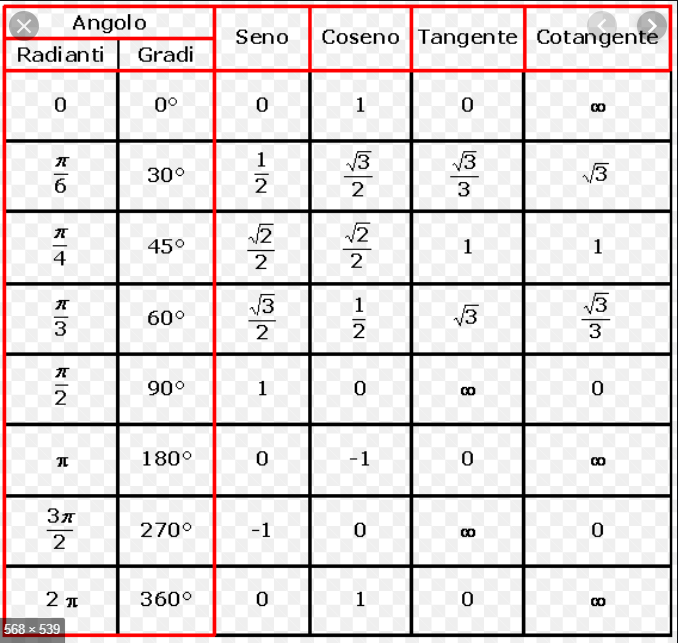
\includegraphics[width=300px]{../capitolo0/trigonometria.PNG}
\end{figure}
\newpage
\subsection{Asintotici}
\begin{figure}[h!]
    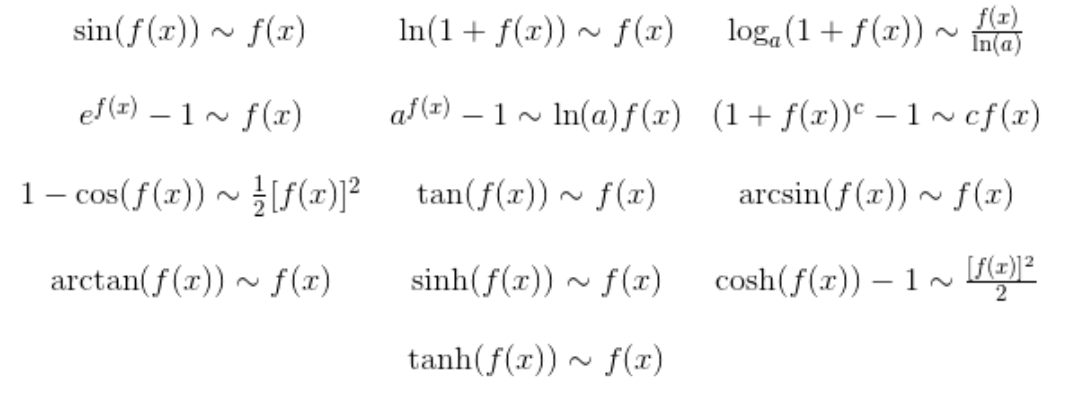
\includegraphics[width=\linewidth]{../capitolo0/asintotici.PNG}
\end{figure}
\newpage
\subsection{Derivate}
\begin{figure}[h!]
    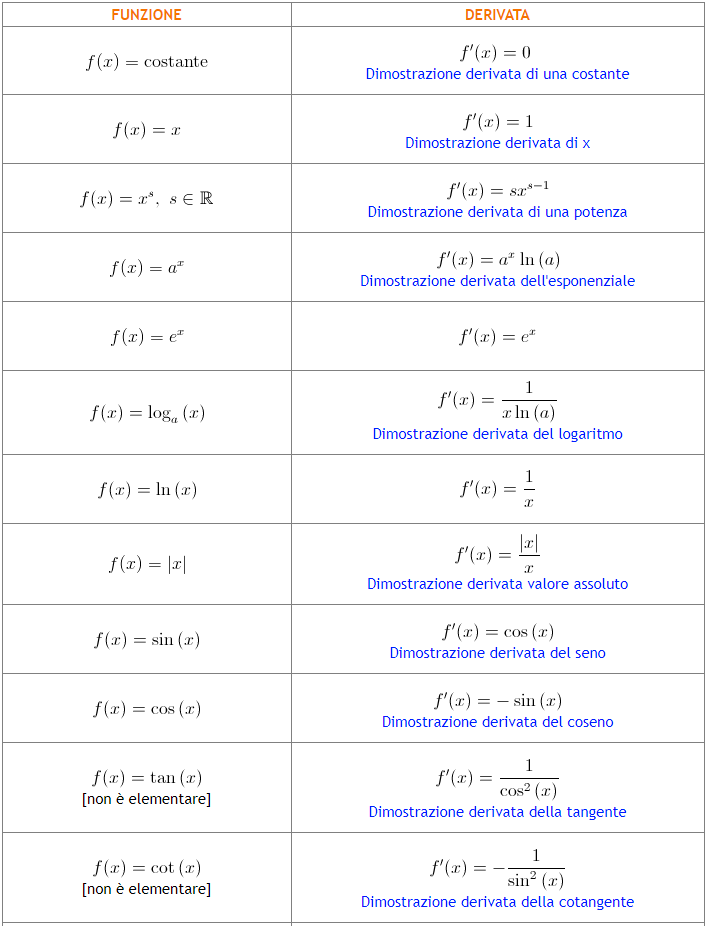
\includegraphics[width=\linewidth]{../capitolo0/derivate1.PNG}
\end{figure}
\newpage
\begin{figure}[h!]
    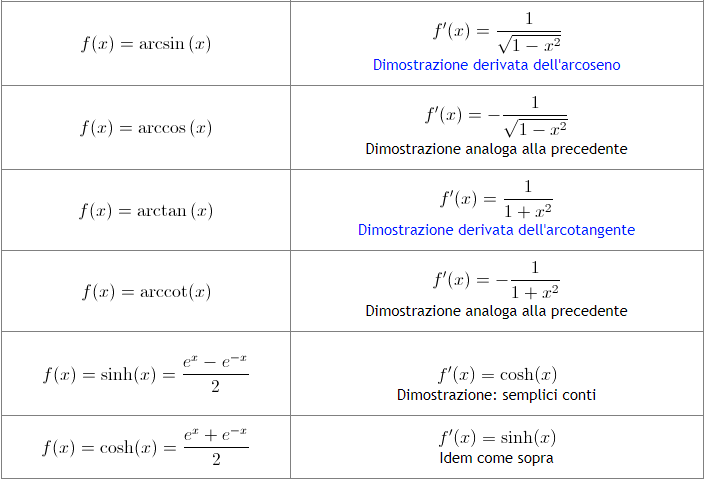
\includegraphics[width=\linewidth]{../capitolo0/derivate2.PNG}
\end{figure}
\newpage
\subsection{Sviluppi}
\begin{figure}[h!]
    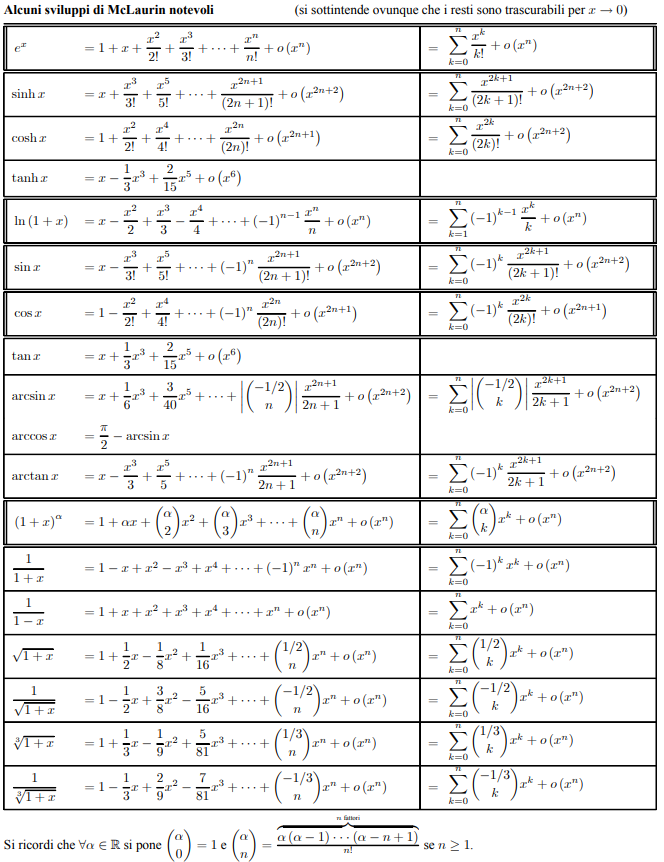
\includegraphics[width=\linewidth]{../capitolo0/mclaurin.PNG}
\end{figure} % ripasso trigonometria, derivate, asintotici, sviluppi di taylor
    \newpage
    \section{Serie}
\subsection{serie geometrica}
\[
    \sum_{n=0}^{\infty}q^n = \begin{cases}
        \frac{1}{1-q} & se \;\; -1<q<1\\
        +\infty &se \;\; q \geq 1\\
        irregolare \;\;& se \;\; q\leq-1 
    \end{cases}
\]
\subsection{serie armonica}
\[
    \sum_{n=1}^{\infty}\frac{1}{n} \geq log(n+1) \rightarrow +\infty
\]
\subsection{serie armonica generalizzata}
\[
    \sum_{n=1}^{\infty} \frac{1}{n^{\alpha}}
\]
per $\alpha \leq 1$ 
\[
    \sum_{n=1}^{\infty} \frac{1}{n^\alpha} \geq \sum_{n=1}^{\infty}\frac{1}{n} \rightarrow +\infty \;\;\;\text{diverge}\;
\]
per $\alpha > 1$ 
\[
    \sum_{n=1}^{\infty} \frac{1}{n^\alpha} = converge
\]
per $\alpha = 2$
\[
    \sum_{n=1}^{\infty}\frac{1}{n^2} = \frac{\pi^2}{6} (\sim  \sum_{n=1}^{\infty} \frac{1}{n(n+1)} = serie \;\; di \;\; mengoli)
\]
\subsection{serie di mengoli}
\[
    \sum_{n=1}^{\infty}\frac{1}{n(n+1)} = \sum_{n=1}^{\infty} \frac{1}{n}-\frac{1}{n+1} = 1- \frac{1}{n+1} \rightarrow 1
\]
\subsection{numero e}
\[
    \lim_{n\rightarrow \infty} \left( 1 + \frac{1}{n} \right)^n = e
\]
\subsection{sviluppi di Taylor delle funzioni elementari}
\[
    e^x = \lim_{n\rightarrow +\infty}\sum_{k=0}^{n} \frac{x^k}{k!} = \sum_{k=0}^{+\infty} \frac{x^k}{k!}
\]
\[
    sin (x) =\sum_{k=0}^{\infty}(-1)^k \frac{x^{2k+1}}{(2k+1)!} =  \frac{e^{ix} - e^{-ix}}{2}
\]
\[
    cos (x) =\sum_{k=0}^{\infty}(-1)^k \frac{x^{2k}}{(2k)!} =\frac{e^{ix} + e^{-ix}}{2}
\]
\subsection{Serie di potenza}
Con $a_k$ costanti reali (o complesse) e $x$ variabile reale (o complessa)
\[
    \sum_{k=0}^{\infty}a_k x^k
\]
\[
    Sh (x) = \sum_{k=0}^{\infty} \frac{x^{2k+1}}{(2k+1)!}
\]
\[
    Ch(x) = \sum_{k=0}^{\infty} \frac{x^{2k}}{(2k)!}
\]
\[
    log(1+x)= \sum_{k=1}^{\infty} (-1)^{k+1} \frac{x^k}{k} \;\;\; per \;\; |x|<1
\]
per $\alpha \in \mathbb{R}$
\[
    (1+x)^\alpha = \sum_{k=0}^{\infty} \binom{\alpha}{k}x^k \;\;\; per \;\; |x|<1
\]
\textbf{teor.} Condizione necessaria affinché una serie $\sum_{n=0}^{\infty} a_n$ converga è che il termine generale $a_n$ tenda a zero. (Cioè perchè la serie converga, il termine $a_n$ deve tendere a zero, ma non per forza se il termine $a_n$ tende a zero allora la serie converge)\newline
\newline
\textbf{teor.}supponiamo che una serie $\sum_{n=0}^{\infty} a_n$ converga, allora per ogni $k$ anche risulta convergente anche $\sum_{n=k}^{\infty} a_n$.\newline
\newline
\textbf{Criterio serie a termini non negativi} Una serie $\sum_{n=0}^{\infty}a_n$ a termini non negativi è convergente o divergente a $+\infty$. Essa converge se e solo se la successione delle somme parziali n-esime è limitata.\newline
\newline
\textbf{Criterio del confronto} Siano $\sum an$ e $\sum b_n$ due serie a termini non negativi tali che $a_n<b_n$ definitivamente, allora:
\begin{itemize}
    \item $\sum b_n$ convergente $\Rightarrow \sum a_n$ convergente. 
    \item $\sum a_n$ divergente $\Rightarrow \sum b_n$ divergente. 
\end{itemize}
\textbf{Criterio del confronto asintotico} Se $a_n \sim b_n$, allora le corrispondenti serie $\sum a_n$ e $\sum b_n$ hanno lo stesso carattere (o entrambe divergenti o entrambe divergenti )\newline
\newline
\textbf{Criterio della radice} Sia $\sum a_n$ una serie a termini non negativi. Se esiste il limite 
\[
    \lim_{n\rightarrow +\infty}\sqrt[n]{a_n} = l
\]
\begin{itemize}
    \item $l>1$ la serie diverge $+\infty$
    \item $l<1$ la serie converge
    \item $l=1$ nulla si può concludere
\end{itemize}
Spesso utilizzato con termini che hanno come esponente $n$.\newline
\newline
\textbf{Criterio del rapporto} Sia $\sum a_n$ una serie a termini positivi. Se esiste il limite 
\[
    \lim_{n\rightarrow +\infty} \frac{a_{n+1}}{a_n} = l
\]
\begin{itemize}
    \item $l>1$ diverge $+\infty$
    \item $l<1$ converge 
    \item $l=1$ nulla si può concludere
\end{itemize}
Spesso utilizzato quando si hanno termini come $n^n$ e $n!$.\newline
\newline
\textbf{Criterio serie a termini di segno variabile} Una serie $\sum a_n$ si dice assolutamente convergente se converge la serie $\sum |a_n|$. Se la serie $\sum a_n$ converge assolutamente, allora converge.\newline
\newline
\textbf{Criterio di Leibniz} Sia data la serie 
\[
    \sum_{n=0}^{\infty}(-1)^n a_n \;\; con  \;\; a_n\geq 0 \;\forall\;n
\]
Se la successione $\{a_n\}$ è decrescente e se $a_n \rightarrow 0$ per $n \rightarrow \infty$, allora la serie è convergente.\newline
Il criterio di Leibniz può essere applicato anche se i termini sono definitivamente di segno alterno e la successione $a_n$ è definitivamente decrescente.\newline
Per verificare la decrescenza bisogna dimostrare che $a_{n+1}<a_n$ oppure mediante il limite a $+ \infty$ della derivata prima di $a_n$ o studiano quando la derivata prima di $a_n<0$ .\newline
Per determinare se una serie è decrescente non vanno usati gli asintotici !\newline
\newline
\textbf{Criterio della somma di serie convergenti} Se $\sum_{n=1}^{\infty} a_n$ converge e $\sum_{n=1}^{\infty} b_n$ converge, allora $\sum_{n=1}^{\infty} a_n +b_n$ converge.\newline
\newline
\textbf{Criterio della somma di serie convergenti e divergenti} Se $\sum_{n=1}^{\infty} a_n$ converge e $\sum_{n=1}^{\infty} b_n$ diverge, allora $\sum_{n=1}^{\infty} a_n + b_n$ diverge.\newline
\newline
\textbf{Criterio serie a termini complessi} Sia la serie $\sum_{n=0}^{\infty} a_n$ con $a_n$ complesso, se la serie  $\sum_{n=0}^{\infty} |a_n|$ converge, allora anche $\sum_{n=0}^{\infty} a_n$ converge \newline
\newline
\textbf{Criterio di Dirichlet} Siano $a_n$ e $b_n$ due succesioni tali che:
\begin{itemize}
    \item $a_n$ è a valori complessi e la sua successione delle somme parziali è limitata.
    \item $b_n$ è a valori reali positivi e tende monotonamente a zero
\end{itemize}
allora la serie $\sum a_nb_n$ è convergente. % serie di analisi 1
    \newpage
    \section{Integrali}
\subsection{Teorema fondamentale del calcolo integrale:}
\[
    \int_{a}^{b} f(x) dx = G(b) - G(a)
\]
\subsection{Proprietà degli integrali:}
\[
    \int_{a}^{b} f(x)dx = \int_{a}^{r} f(x) dx + \int_{r}^{b} f(x) dx
\]
\[
    \left| \int_{a}^{b} f(x) dx \right| \leq \int_{a}^{b} |f(x)| dx
\]
\[
    \int k \cdot f(x) dx = k \cdot \int f(x) dx
\]
\[
    \int [f_1(x) + f_2(x) ] dx= \int f_1(x) dx + \int f_2(x) dx
\]
\subsection{Integrali fondamentali:}
\[
    \int f'(x) dx = f(x) +c
\]
\[
    \int a \; dx = ax +c
\]
\[
    \int x^n dx = \frac{x^{n+1}}{n+1} +c
\]
\[
    \int \frac{1}{x}dx = ln(|x|) +c
\]
\[
    \int sin(x) dx = -cos(x) +c
\]
\[
    \int cos(x) dx = sin(x)+c
\]
\[
    \int tan(x) dx = -log|cos(x)| +c
\]
\[
    \int log(x) dx \;\; = xlog(x) - \int x \cdot  \frac{1}{x} dx - \int 1 dx = x log(x) -x + c
\]
\[
    \int arctg (x) dx \;\; = x arctg(x) -\int \frac{x}{1+x^2}dx = x arctg(x) -\frac{1}{2}log(1+x^2) + c 
\]
\[
    \int cotg(x) dx = log|sin(x)| +c
\]
\[
    \int (1+tg^2(x))dx = \int \frac{1}{cos^2(x)} dx = tg(x) +c
\]
\[
    \int (1+ctg^2(x))dx = \int \frac{1}{sin^2(x)} dx = -cotg(x) +c
\]
\[
    \int Sh(x) dx = Ch(x) +c
\]
\[
    \int Ch(x) dx = Sh(x) +c
\]
\[
    \int Th(x) dx = log(Ch(x))+c
\]
\[
    \int Coth(x) dx = log|Sh(x)| +c
\]
\[
    \int e^x dx = e^x+c
\]
\[
    \int e^{kx} dx = \frac{e^{kx}}{k} +c
\]
\[
    \int a^x dx = \frac{a^x}{ln(a)}+c
\]
\subsection{Integrali notevoli:}
\[
    \int sin^2(x) dx = [integrato \; una \; volta \; per \; parti \; e \; sostituzione \; con \; cos^2(x)+ sin^2(x) = 1] = \frac{1}{2}(x-sin(x)cos(x)) +c
\]
\[
    \int cos^2(x) dx = [integrato \; una \; volta \; per \; parti \; e \; sostituzione \; con \; cos^2(x)+ sin^2(x) = 1] = \frac{1}{2}(x+sin(x)cos(x)) +c
\]
\[
    \int tan^2(x) dx = tan(x) -x +c
\]
\[
    \int cotan^2(x) dx = -x -cot(x) +c 
\]
\[
    \int Sh^2(x) dx = [integrato \; una \; volta \; per \; parti \; e \; sostituzione \; con \; Ch^2(x) - Sh^2(x) = 1] = \frac{1}{4}(Sh(2x)-2x) +c
\]
\[
    \int Ch^2(x) dx = [integrato \; una \; volta \; per \; parti \; e \; sostituzione \; con \; Ch^2(x) - Sh^2(x) = 1] = \frac{1}{2}(x + Sh(x)Ch(x)) +c
\]
\[
    \int Th^2(x) dx = x - Th(x) +c 
\]
\[
    \int Coth^2(x) dx = x - Coth(x) +c 
\]
\[
    \int \frac{1}{sin^2(x)} dx = [1 = cos^2(x) +sin^2(x)] = \int 1 + tan^2(x) dx = -cotan(x) + c
\]
\[
    \int \frac{1}{cos^2(x)} dx = [1 = cos^2(x) +sin^2(x)] = \int 1 + cotan^2(x) dx = tan(x) + c
\]
\[
    \int \frac{1}{tan^2 (x)} dx = \int cotan^2(x) dx 
\]
\[
    \int \frac{1}{cotan^2(x) }dx = \int tan^2(x) dx 
\]
\[
    \int \frac{1}{Ch^2(x)} dx = \int (1-Th^2(x))dx= Th(x)+c
\]
\[
    \int \frac{1}{Sh^2(x)} = \int (-1 Coth^2(x)) dx = -Coth(x) +c
\]
\[
    \int \frac{1}{1+x^2} dx = arctg(x) +c
\]
\[
    \int \frac{1}{1-x^2} dx = \frac{1}{2}log\left|\frac{1+x}{1-x}\right|+c
\]
\[
    \int \frac{1}{\sqrt{1+x^2}} dx = arcSh(x) +c = log(x + \sqrt{1+x^2}) +c
\]
\[
    \int \frac{1}{\sqrt{1-x^2}} dx = arcsin(x) +c
\]
\[
    \int \frac{1}{\sqrt{-1 + x^2}} dx = log|x+ \sqrt{x^2-1}| +c
\]
\[
    \int \frac{1}{\sqrt{\pm a^2 + x^2}} dx = log|x + \sqrt{x^2 \pm a^2}|+c
\]
\[
    \int \sqrt{x^2 \pm a^2} dx = \frac{x}{2} \sqrt{x^2 \pm a^2} \pm \frac{a^2}{2} log(x + \sqrt{x^2 \pm a^2}) +c
\]
\[
    \int \sqrt{a^2 - x^2}dx = \frac{1}{2}(a^2arcsin(\frac{x}{a}) + x \sqrt{a^2 - x^2} )+c
\]
\subsection{Integrali riconducibili:}
\[
    \int f^n(x) \cdot f'(x) dx = \frac{f^{n+1}(x)}{n+1} +c
\]
\[
    \int \frac{f'(x)}{f(x)} dx = log|f(x)|+c
\]
\[
    \int f'(x) \cdot cos(f(x)) dx =  sin(f(x))+c
\]
\[
    \int f'(x) \cdot sin(f(x)) dx = -cos(f(x)) +c
\]
\[
    \int e^{(f(x)} \cdot f'(x) dx = e^{f(x)}+c
\]
\[
    \int a^{f(x)} \cdot f'(x) dx = \frac{a^{f(x)}}{ln(a)} +c
\]
\[
    \int \frac{f'(x)}{1+f^2(x)} dx = arctg(f(x))+c
\]
\subsection{Integrazione per sostituzione:}
Sostituire alla variabile $x$ una funzione di un'altra variabile $t$, purchè tale funzione sia derivabile e invertibile.\newline
Ponendo $x = g(t)$ da cui deriva $dx = g'(t) dt$ si ha che:
\[
    \int f(x) dx = \int f[g(t)] \cdot g'(t) dt
\]
Da ricordare è che se si è in presenza di un integrale definito bisogna aggiornare anche gli estremi di integrazione. Se non si volesse cambiare l'intervall odi integrazione si può risostituire il vecchio valore di $t$.
\subsection{Integrazione delle funzioni razionali:}
\[
    \int \frac{P_n(x)}{Q_m(x)} dx
\]
Per prima cosa se il grado del numeratore è $\geq$ del grado del denominatore, si esegue la divisione di polinomi:
\begin{itemize}
    \item Si dispongono i polinomi dal termine di grado maggiore a quello minore nella seguente maniera:
    \[
        P(x) \;\; | \;\; Q(x)    
    \]
    badando al fatto che se nel polinomio $P(x)$ mancasse qualche termine bisognerebbe scrivere $0$ nella sua posizione.
    \item Si dividono il termine di grado massimo di $P(x)$ con quello di grado massimo di $Q(x)$, riportando il risultato al di sotto di $Q(x)$.
    \item Moltiplichiamo il termine appena scritto per ogni termine di $Q(x)$, ne invertiamo il segno e lo trascriviamo al di sotto dei termini con lo stesso grado di $P(x)$
    \item Sommiamo termine per termine $P(x)$ con i valore appena scritti e li riportiamo sotto.
    \item Ripetiamo questo procedimento finchè il grado più alto fra i termini dell'ultima riga scritta a sinistra è minore (non minore uguale) del termine di grado massimo di $Q(x)$
    \item Il polinomio a destra è il risultato della divisione $S(x)$, mentre ciò che rimane sulla sinistra è il resto $R(x)$. Possiamo ora riscrivere il numeratore:
    \[
        P(x) = S(x) \cdot Q(x) + R(x)
    \]
\end{itemize}
Vediamo ora i vari casi possibili:
\begin{itemize}
    \item \textbf{denominatore di primo grado:} integrale immediato tramite il logaritmo
    \item \textbf{denominatore di secondo grado:} si calcola il segno del discriminante:
    \begin{itemize}
        \item \textbf{due radici distinte:} si scompone in fratti semplici
        \[
            \frac{N(x)}{D_1(x) \cdot D_2(x)} = \frac{a}{D_1(x)} + \frac{b}{D_2(x)}
        \]
        \[
            \frac{a \cdot D_2(x) + b \cdot D_1(x)}{D_1(x) \cdot  D_2(x)} = \frac{N(x)}{D_1(x) \cdot D_2(x)}
        \]
        \[
            a \cdot D_2(x) + b \cdot D_1(x)= N(x)
        \]
        Una volta determinate $a$ e $b$ si riscrive l'integrale come $\frac{a}{D_1(x)} + \frac{b}{D_2(x)}$ e si integra come somma di logaritmi
        \item \textbf{denominatore quadrato perfetto:} (due soluzioni coincidenti), si procede per sostituzione:
        \[
            \int \frac{N(x)}{D(x)^2} dx = [D(x) = t, \; \dots] = \; \dots
        \] 
        L'utilità della sostituzione è quella di spezzare la frazione in una somma di frazion ida integrare una ad una.
        \item \textbf{denominatore non si annulla mai:}\newline
        Casi semplici:
        \[
            \int \frac{1}{1 + x^2}dx = arctg (x) +c
        \]
        \[
            \int \frac{1}{x^2 + a^2}dx = \frac{1}{a} arctg \frac{x}{a} +c
        \]
        \[
            \int \frac{1}{a^2 + (x+b)^2}dx = \frac{1}{a} arctg \frac{x+b}{a} +c
        \]
        Caso generico: Si cerca di dividere l'integrale in una somma di integrali, il primo deve contenere al numeratore la derivata del denominatore, il secondo non deve contenere la $x$ al numeratore, cioè deve essere una costante e quindi riconducibile ai casi semplici sopra riportati. Il denominatore non cambia. Ci si arriva a logica. 
    \end{itemize}
    \item \textbf{denominatore di grado maggiore di due:} è sempre possibile scomporlo in prodotti di fattori di primo grado o di secondo grado irriducibili, per farlo si usa Ruffini (o altrimenti si va a tentoni ricordando che PROBABILMENTE una radice della funzione è un dividendo (positivi e negativi) del numero che si ricava moltiplicando il coefficiente del termine massimo e il termine noto).\newline
    Fatto questo si scompone la frazione in fratti semplici con la stessa logica del caso di due radici distinte, ricordando che il numeratore deve essere un espressione di un grado minore del denominatore, per esempio se il denominatore è di grado $2$, allora si userà $ax+b$ che è di grado $1$.
\end{itemize}
\subsection{Funzioni razionali di $e^x$}
Si pone $e^x = t$, $x= log(t)$, $dx = \frac{dt}{t}$ e ci si riconduce a una funzione razionale classica.
\subsection{Integrazione per parti:}
\[
    \int f'(x) \cdot  g(x) dx = f(x) \cdot g(x) - \int f(x) \cdot g'(x)dx
\]
La formula deriva dalla formula di derivazione della moltiplicazioni di due funzioni:
\[
    (fg)' = f'g + fg'
\]
\[
    fg' = (fg)' - f'g
\]
Si può vedere la formula di integrazione per parti più facilmente così:
\[
    \int integranda \cdot derivanda \; dx = primitiva \cdot derivanda - \int primitiva \cdot derivata \; dx
\]
L'integrazione per parti si usa:
\begin{itemize}
    \item dovendo calcolare integrali della forma
    \[
        \int x^n \cdot f(x) dx \;\;\; f(x) = \begin{cases}
            cos(x)\\ 
            sin(x)\\ 
            e^x\\ 
            Sh(x)\\ 
            Ch(x)        
        \end{cases}
    \]
    si integra per parti derivando $x^n$ e integrando $f(x)$. Per $n=1$ l'integrale si riduce a uno immediato, per $n>1$ si itera il procedimento fino al caso $n=1$. Si possono svolgere allo stesso modo anche integrali del tipo:
    \[
        \int P_n(x) f(x) dx
    \]
    \item dovendo calcolare integrali della forma
    \[
        \int f(x) g(x) dx \;\;\;\; \begin{cases}
            f(x) = e^{\alpha x}, Sh(\alpha x), Ch( \alpha x), a^{bx} \\
            g(x) = cos( \beta x), sin(\beta x)
        \end{cases}
    \]
    si eseguono due integrazioni per parti consecutive, nella prima la scelta della funzione da integrare o derivare è indifferente, nella seconda però la scelte deve essere coerente alla prima. Chiamando $I$ l'integrale di partenza si ottiene una funzione della forma
    \[
        I = h(x) - \frac{\beta}{\alpha}^2 I
    \]
    da cui si ricava $I$.\newline
    Se entrambe le funzioni $f(x)$ e $g(x)$ sono del tipo $cos(x)$ o $sin(x)$ si usano le formule di duplicazione o prostaferesi (vedi più avanti).
    \item L'integrale del logaritmo, derivando $log(x)$ e integrando $1$
    \[
        \int log(x) dx \;\; = xlog(x) - \int x \cdot  \frac{1}{x} dx - \int 1 dx = x log(x) -x + c
    \]
    Più in generale, dovendo calcolare integrali della forma
    \[
        \int x^m log^n(x) dx
    \]
    e ponendo $g' = x^m$ e $f = log^n(x)$ ed eseguendo iterativamente $n$ integrazioni per parti si riesce a calcolare l'integrale del logaritmo. Ancora più in generale si possono risolvere integrali della forma:
    \[
        \int P_m(x) \cdot Q_n(log(x)) dx 
    \]
    \item l'integrale dell'arcotangente, derivando $arctg(x)$ e integrando $1$
    \[
        \int arctg (x) dx \;\; = x arctg(x) -\int \frac{x}{1+x^2}dx = x arctg(x) -\frac{1}{2}log(1+x^2) + c 
    \]
    Più in generale
    \[
        \int x^n arctg(x) dx  = \frac{x^{n+1}}{n+1}arctg(x) - \int\frac{x^{n+1}}{n+1} \frac{dx}{1+x^2}
    \]
\end{itemize}
\subsection{integrazione delle funzioni trigonometriche}
\begin{itemize}
    \item dovendo calcolare
    \[
        \int f(sin(x)) \cdot  cos(x) dx \;\;\; \Rightarrow  \;\;\; sin(x) = t, cos(x) dx =dt
    \]
    \[
        \int f(cos(x)) \cdot  sin(x) dx\;\;\; \Rightarrow  \;\;\; cos(x) ) t, -sin(x) dx = dt
    \]
    In particolare per calcolare 
    \[
        \int sin^n(x) cos^m(x)
    \]
    se almeno uno degli esponenti è dispari si riesce a riscrivere l'integrale in una delle forme viste sopra utilizzando: $sin^2(x) + cos^2(x) = 1$. Se entrambi gli esponenti sono pari si usano le formule trigonometriche per abbassarne il grado: $cos^2(x) = \frac{1}{2}(1+cos(2x))$ e $sin^2(x) = \frac{1}{2} (1-cos(2x))$
    \item per integrali del tipo
    \[
        \int cos(\alpha x) sin(\beta x) dx, \;\;\;\int cos(\alpha x) cos(\beta x) dx, \;\;\;\int sin(\alpha x) sin(\beta x) dx,
    \]
    si usano le regole di prostaferesi che riconducono a somme di integrali immediati
    \item integrali di funzioni razionali di $sin(x)$ e $cos(x)$ possono sempre essere ricondotti a integrali di funzioni razionali generiche tramite la sostituzione:
    \[
        t = tg\left(\frac{x}{2}\right), \;\;\; x= 2 arctg(t), \;\;\;dx = \frac{2}{1+t^2}dt
    \]
    ne derivano le seguenti identità trigonometriche:
    \[
        \begin{cases}
            cos(x) = \frac{1-t^2}{1+t^2}\\
            sin(x) = \frac{2t}{1+t^2}
        \end{cases}
    \]
    \item integrali definiti notevoli:
    \[
        \int_{0}^{n \frac{\pi}{2}}cos^2(kx) dx = \int_{0}^{n \frac{\pi}{2}}sin^2(kx) dx = n \frac{\pi}{4}
    \]
    \item per calcolare integrali razionali con $Sh(x)$ e $Ch(x)$ o si trovano scorciatoie con trasformazioni oppure si usa la sostituzione $e^x = t, x= log(t), dx = \frac{dt}{t}$
\end{itemize}
\subsection{Integrazione delle funzioni irrazzionali}
\begin{itemize}
    \item se l'integranda è una funzione razionale di $x$ moltiplicata per solo una delle seguenti
    \[
        \int R(x) \sqrt{a^2-x^2} dx = [x=a \cdot  sin(t), dx =a \cdot  cos(t)dt] = \int \sqrt{a^2(1-sin^2(t))}dx = \int|a \cdot  cos(t)|dx
    \]
    \[
        \int R(x) \sqrt{a^2 + x^2} = [x=a \cdot  Sh(t), dx =a \cdot  Ch(t)dt] = \int \sqrt{a^2(1-Sh^2(t))}dx = \int a \cdot  Ch(t)dx
    \]
    \[
        \int R(x) \sqrt{x^2 -a^2} = [x=a \cdot  Ch(t), dx =a \cdot Sh(t)dt] = \int \sqrt{a^2(Ch^2(t)-1)}dx = \int|a \cdot Sh(t)|dx
    \]
    Negli ultimi due casi per tornare alla variabile x occorre usare le funzioni iperobliche inverse:
    \[
        \begin{cases}
            x = a \cdot  Ch(t) \Rightarrow t = SettCh(\frac{x}{a}) = log\left(\frac{x}{a}+\sqrt{\frac{x^2}{a^2}-1}\right)\\
            x= a \cdot Sh(t) \Rightarrow t = SettSh\left(\frac{x}{a}\right) = log\left(\frac{x}{a}+\sqrt{\frac{x^2}{a^2}+1}\right)
        \end{cases}
    \]
    è utile anche ricordare che $Sh(SettCh(a))= \sqrt{a^2-1}$ e $Ch(SettSh(a))=\sqrt{a^2+1}$
    \item integrale di una funzione razionale di $x, x^{\frac{n_1}{m_1}}, x^{\frac{n_2}{m_2}}$, etc. \newline
    Si pone $x = t^n$ con $n=$ minimo comune multiplo di $m_1$, $m_2$, etc. Si ha quindi $dx = n \cdot  t^{n-1} dt$ e si ottiene una funzione razionale di $t$.
    \item Se l'integranda è una funzione del tipo $R(x^{2n+1}, \sqrt{x^2 \pm a^2})$
    \[
        \int x^{2n+1}R(\sqrt{x^2 \pm a^2})dx = [\sqrt{x^2 \pm a^2} = t, xdx= tdt, x^{2n+1} \cdot dx = (t^2 \mp a^2)^n t \cdot  dt]
    \]
\end{itemize}
\subsection{Simmetrie e valori assoluti nel calcolo di integrali definiti}
\begin{itemize}
    \item se $f(x)$ è \textbf{pari}:
    \[
        \int_{-k}^{k}f(x)dx = 2 \int_{0}^{k} f(x) dx
    \]
    \item se $f(x)$ è \textbf{dispari}:
    \[
        \int_{-k}^{k}f(x)dx = 0
    \]
\end{itemize}
\subsection{Osservazione. Integrale generalizzato di una funzioen dispari su un intervallo simmetrico}
Non è corretto affermare l'annullarsi di un integrale dispari per motivi di simmetria in un intervallo simmetrico senza prima verificare la convergenza dell'integrale stesso.
\subsection{INTEGRALI GENERALIZZATI}
\subsection{Integrazione di funzioni non limitate}
Metodo generale di risoluzione:
\[
    \lim_{x\rightarrow b^-} f(x) = \pm \infty \;\;\;\;\;\;\;\;\;\;\;\;\;\;\;\;\;\;\;\;\;\;\;\;\;\;\;\;\;\;\;\;\;\;\;\;\;\;\;\;\lim_{x\rightarrow a^+}f(x) = \pm \infty
\]
\[
    \int_{a}^{b}f(x)dx = \lim_{\epsilon\rightarrow 0^+}\int_{a}^{b-\epsilon}f(x)dx \;\;\;\;\;\;\;\;\;\;\;\;\; \int_{a}^{b}f(x)dx = \lim_{\epsilon\rightarrow 0^+}\int_{a+\epsilon}^{b}f(x)dx 
\]
\subsection{Criteri di integrabilità al finito}
Siano $\lim_{x\rightarrow b^-}f(x) = \lim_{x\rightarrow b^-}g(x) = + \infty$:
\begin{itemize}
    \item confronto: se $0\leq f(x) \leq g(x)$, allora $g$ integrabile $\Rightarrow f$ integrabile e $f$ non integrabile $\Rightarrow g$ non integrabile.
    \item confronto asintotico: se $f>0$ e $g>0$ e $f \sim g$ per $x \rightarrow b^-$, allora $f$ integrabile $\Leftrightarrow g$ integrabile.
    \item \textbf{teor.} (da usare per studiare per esempio funzioni seno e coseno per $x \rightarrow \infty$)
    \[
        \int_{a}^{b}|f(x)|dx \;\; convergente \;\;\Rightarrow \int_{a}^{b}f(x)dx \;\;convergente
    \]
\end{itemize}
\subsection{Integrazione su intervalli illimitati}
Metodo generale di risoluzione:
\[
    \int_{a}^{+\infty}f(x) dx = \lim_{\omega\rightarrow +\infty}\int_{a}^{\omega}f(x)dx
\]
\[
    \int_{- \infty}^{b}f(x) dx = \lim_{\omega\rightarrow -\infty}\int_{\omega}^{b}f(x)dx
\]
\[
    \int_{-\infty}^{+\infty}f(x) dx = \int_{-\infty}^{c} f(x) dx + \int_{c}^{+\infty}f(x) dx
\]
\textbf{def.} Se il limite dell'integrale di $f$ esiste finito allora $f$ si dice integrabile oppure che l'integrale è convergente. \newline
\textbf{def.} Se il limite dell'integrale è $\pm \infty$, l'integrale si dice divergente.\newline
\textbf{def.} Se il limite non esiste, l'integrale non esiste.\newline
\textbf{per essere integrabile deve avere limite finito.}
\subsection{Criteri di integrabilità all'infinito}
\begin{itemize}
    \item confronto: se $0\leq f(x) \leq g(x)$ in $[a,+\infty)$, allora $g$ integrabile $\Rightarrow f$ integrabile e $f$ non integrabile $\Rightarrow g$ non integrabile.
    \item confronto asintotico: se $f>0$, $g>0$ e $f \sim g$ per $x \rightarrow + \infty$, allora $f$ integrabile $\Leftrightarrow g$ integrabile
    \item \textbf{teor.} (da usare per studiare per esempio funzioni seno e coseno per $x \rightarrow \infty$)
    \[
        \int_{a}^{+\infty}|f(x)| dx \;\; convergente \;\; \Rightarrow \int_{a}^{+\infty} f(x) dx \;\;convergente
    \]
\end{itemize}
\subsection{Osservazione. Ordine di annullamento di una funzione derivabile.}
Se $f$ è una funzione derivabile in un intervallo $I$, la formula di Taylor ci dice che se $f$ si annulla in un punto $\alpha \in I$, si annulla almeno del prim'ordine. Precisamente poichè
\[
    f(x) - f(\alpha) = f'(\alpha)(x-\alpha) + o(x-\alpha)
\]
se $f'(\alpha) \neq 0$ allora $f$ ha uno zero del prim'ordine in $\alpha$. Se $f'(\alpha) = 0$ ma, ad esempio, $f''(\alpha) \neq 0$, si può concludere che $f$ si annulla del $2^0$ ordine, e così via. In ogni caso non può annullarsi di un ordine inore di $1$.
\subsection{Integrali generalizzati notevoli}
Caso 1:
\[
    \int_{a}^{b}\frac{1}{(x-a)^p}dx \rightarrow \begin{cases}
        converge \;\;&se \;\;p<1\\
        diverge \;\;&se \;\; p\geq 1
    \end{cases}
\]
\[
    \int_{a}^{b}\frac{dx}{(b-x)^p} \rightarrow  \begin{cases}
        converge \;\;&se \;\;p<1\\
        diverge \;\;&se \;\; p\geq 1
    \end{cases}
\]
Caso 2:
\[
    \int_{a}^{+\infty}\frac{1}{x^p}dx \rightarrow \begin{cases}
        converge \;\; & se \;\; p > 1\\
        diverge \;\; &  se \;\; p \leq 1
    \end{cases}
\]
Caso 3: con $0< \alpha < 1$
\[
    \int_{0}^{\alpha} \frac{1}{x^a \cdot  |ln(x)|^b} \rightarrow \begin{cases}
        converge \;\; se \;\; & \begin{cases}
            a < 1 \;\; e \;\; b \in \mathbb{R}\\
            oppure \\
            a=1 \;\; e \;\; b > 1
        \end{cases}\\
        diverge \;\; se \;\; & \begin{cases}
            a>1 \;\; e \;\; b \in \mathbb{R}\\
            oppure\\
            a=1 \;\; e \;\; b \leq 1
        \end{cases}
    \end{cases}
\]
Caso 4: con $\alpha > 1$
\[
    \int_{\alpha}^{+\infty} \frac{1}{x^\alpha \cdot ln^b(x)}dx \rightarrow \begin{cases}
        converge \;\; se \;\; & \begin{cases}
            a > 1 \;\; e \;\; b \in \mathbb{R}\\
            oppure \\
            a=1 \;\; e \;\; b > 1
        \end{cases}\\
        diverge \;\; se \;\; & \begin{cases}
            a<1 \;\; e \;\; b \in \mathbb{R}\\
            oppure\\
            a=1 \;\; e \;\; b \leq 1
        \end{cases}
    \end{cases}
\]
Caso 5: con $\alpha> 1$
\[
    \int_{1}^{\alpha}\frac{1}{ln^p(x)} dx \rightarrow \begin{cases}
        converge \;\; se \;\; &p<1\\
        diverge \;\; se \;\; &p\geq 1
    \end{cases}
\]
\subsection{FUNZIONI INTEGRALI}
\textbf{teor.} Secondo teorema fondamentale del calcolo integrale \newline
Sia $f: [a,b] \rightarrow \mathbb{R}$ una funzione integrabile e sia $x_0 \in [a,b]$ e sia 
\[
    F(x) = \int_{x_0}^{x} f(t) dt
\]
Allora:
\begin{itemize}
    \item La funzione $F$ è continua in $[a,b]$
    \item Se inoltre $f$ è continua in $[a,b]$, allora $F$ è derivabile in $[a,b]$ e vale
    \[
        F'(x) = f(x) \;\; per \; ogni \; x \in[a,b]
    \]
    (Se $f(t)$ non è continua su tutto $I$, ma è integrabile in senso generalizzato, in tutti i punti in cui $f(t)$ è continua, $F(x)$ è derivabile e $F'(x) = f(x)$)\newline
    $F$ ha punti di non derivabilità dove $f$ è discontinua.
\end{itemize}
Conseguenze:
\begin{itemize}
    \item se $f$ è continua, $F$ è derivabile con continuità
    \item se $f$ è continua e derivabile con continuità, anche $F'$ è derivabile con continuità, quindi $F$ è due volte derivabile con continuità. Iterando: la funzione integrale ha sempre un grado di regolarità in più rispetto alla funzione integranda
    \item ogni fuzione continua su $I$ ha una primitiva su $I$
\end{itemize}
Logica degli esercizi in cui bisogna trovare l'intervallo di definizione:
\[
    F(x) = \int_{x_0}^{x}f(x)dx
\]
\begin{itemize}
    \item lo scopo è determinare dove la funzione integranda è integrabile.
    \item Vedere dove la funzione integranda è continua, una funzione continua è integrabile. Analizzare i punti di discontinuità:
    \item Se una funzione ha un numero finito di discontinuità limitate in un intervallo, allora è integrabile in quell'intervallo. In poche parole se è una discontinuità a salto è integrabile.
    \item Per gli altri punti di discontinuità la funzione integranda è illimitat, quindi bisogna studiarla (con i criteri del confronto, del confronto asintotico, col teorema del modulo, calcolando effettivamente la primitiva e il limite, o riducendosi al caso particolare delle funzioni non limitate con gli asintotici o gli sviluppi di Taylor).
    \item Se la funzione itegranda non è integrabile nel punto $x_0$ allora l'insieme di definizione di $F$ è vuoto. Ma se $x_0$ fosse un punto di accumulazione bisogna studiare l'integrale della funione per $t \rightarrow x_0$ e vedere se è effettivamente integrabile o meno.
\end{itemize}
Logica degli esercizi sulla regolarità delle funzioni integrali:
\[
    F(x) = \int_{x_0}^{x} f(x)dx
\]
\begin{itemize}
    \item si determina l'insieme di definizione. (vedi sopra)
    \item per determinare i punti di non derivabilità di $F(x)$ studiamo la sua derivata $F'(x) = f(x)$. I punti di non derivabilità sono quelli quelli dove $f(x)$ non è definita, e in $F(x)$ corrispondono a:
    \begin{itemize}
        \item discontinuità a salto in $f$ è un punto angoloso in $F$
        \item punti di asintoto verticale di $f$ sono cuspidi (verso l'alto o il basso) o flessi a tangente verticale (ascendente o discendente) di $F$
    \end{itemize}
    \item Notiamo che tangenti verticali o discontinuità a salto o buchi nella funzione di $F$ non possono essere presenti nel dominio di $F$, perchè essendo punti di discontinuità non sono derivabili e dunque non presenti nell'intervallo di integrazione di $f$.\newline
    Dunque la funzione $F$ è (sempre) continua nel suo intervallo di definizione.
\end{itemize}
Logica degli esercizi sui grafici qualitativi della funzione integrale $F(x)$ a partire dalla funzione integranda $g(x)$
\begin{itemize}
    \item $F$ è crescente sugli intervalli in cui $g$ è positiva, $F$ è decrescente sugli intervalli in cui $g$ è negativa.
    \item punti in cui $g$ incrocia l'asse delle $x$ sono punti di massimo o minimo
    \item discontinuità a salto in $g$ sono punti angolosi
    \item $F$ è concava verso l'alto (il basso) negli intervalli in cui $g$ è crescente (decrescente)
    \item punti di cambio massimo e minimo in $g$ sono punti di cambio di concavità in $F$
\end{itemize}
Limite all'infinito di una funzione integrale:
\[
    \lim_{x\rightarrow +\infty}F(x) = \; integrale \;\;generalizzato \;\;= \int_{x_0}^{+\infty}f(t)dt
\]
se l'integrale generallizzato converge esiste limite finito (anche se non si riesce a calcolare), se non converge o è divergente o non esiste.\newline
Caso particolare è quello in cui $f(t) \rightarrow m$, costante non nulla, per cui $F(x) \sim  mx$. Quindi $F(x)$ tende a infinito con crescita lineare e potrebbe avere asintoto obliquo calcolabile come 
\[
    \lim_{x\rightarrow \infty}[F(x)-mx] = \lim_{x\rightarrow \infty}\int_{x_0}^{x}[f(t)-m]dt + mx_0
\]
Ossia esiste asintoto obliquo se l'integrale generalizzato
\[
    \int_{x_0}^{\infty}[f(t)-m]dt
\]
converge. % integrali di analisi 1
    \newpage
    \section*{2-Calcolo infinitesimale per le curve}
\rule{\textwidth}{2pt}
\subsection*{Richiami di calcolo vettoriale}
vettore
\[
    \vec{x} = (x_1, x_2, \dots, x_n)
\]
modulo di un vettore
\[
    |\vec{x}| = \sqrt{\sum_{i=1}^{n}x_i^2}
\]
versore
\[
    vers(\vec{x}) = \frac{\vec{x}}{|\vec{x}|}
\]
$\vec{x}, \vec{y}$ sono paralleli se
\[
    \lambda \vec{x} = \mu \vec{y}\;\; \text{ per qualche } \;\;\lambda, \mu \in \mathbb{R}
\]
Somma di vettori: si sommano le componenti simili.\newline
Prodotto fra un vettore e uno scalare: si moltiplica ogni componente per lo scalare.\newline
Prodotto scalare fra vettori: ha come risultato un numero reale ottenuto dalla formula $\vec{u} \cdot \vec{v} = (u_1 v_1 + u_2 v_2 + \dots + u_n v_n)$. Il prodotto scalare può essere espresso anche come
\[
    \vec{u} \cdot \vec{v} = |\vec{u}| |\vec{v}| cos(\theta)
\]
dove $\theta$ rappresenta l'angolo tra i due vettori. Di conseguenza $\vec{u} \cdot  \vec{v} = 0$ solo se i due vettori sono ortogonali.\newline
Dal prodotto scalare si può ricavare l'angolo fra due vettori
\[
    cos(\theta) = \frac{\vec{u} \cdot  \vec{v} }{|\vec{u}| |\vec{v}|}
\]
Inoltre $\vec{v} \cdot  \vec{v} = |\vec{v}|^2$.\newline
Prodotto vettoriale:
\[
    \vec{u}\text{x}\vec{v} = \left|\begin{matrix}
        i \;\; & j \;\;& k \;\;\\
        u_1 & u_2 & u_3\\
        v_1 & v_2 & v_3\\
    \end{matrix}\right|
\]
Il prodotto vettoriale si annulla solo se i vettori sono paralleli.\newline
Inoltre $\vec{v} \text{x} \vec{v} = 0$.\newline
Prodotto misto:
\[
    \vec{u} \cdot (\vec{v} \text{x} \vec{w}) = \left|\begin{matrix}
        u_1 \;\;& u_2 \;\;& u_3\\
        v_1 &v_2 & v_3\\
        w_1 &w_2 & w_3
    \end{matrix}\right|
\]
Il prodotto misto si annulla solo se i tre vettori sono linearmente indipendenti.\newline
\rule{\textwidth}{2pt}
\subsection*{Funzioni a valori vettoriali, limiti e continuità}
Si dice funzione a valori vettoriali una funzione $\vec{f} : \mathbb{R} \rightarrow  \mathbb{R}^n$ con $n > 1$. Le funzioni $\vec{f} : \mathbb{R} \rightarrow \mathbb{R}^2$ o $\mathbb{R}^3$.\newline
Il limite della funzione a valori vettoriali si calcola componente per componente:
\[
    \lim_{t\rightarrow t_0}(r_1(t), r_2(t), \dots, r_n(t)) = \left(\lim_{t\rightarrow t_0}r_1(t), \lim_{t\rightarrow t_0}r_2(t), \dots, \lim_{t\rightarrow t_0}r_n(t)\right)
\]
Valgono allo stesso modo delle funzioni unidimensionali il teorema di unicità del limite e la definizione di continuità (una funzione a valori vettoriali è continua in un punto se lo sono tutte le sue componenti).\newline
\rule{\textwidth}{2pt}
\subsection*{Curve regolari e calcolo differenziale vettoriale}
Nel caso $n = 2$ o $3$, una funzione $\vec{f} : \mathbb{R} \rightarrow  \mathbb{R}^n$ rappresentano curve nel piano o nello spazio tridimensionale.\newline
Sia $I$ un intervallo in $\mathbb{R}$. Si dice arco di curva continua, o cammino, in $\mathbb{R}^n$ una funzione $\vec{r}: I \rightarrow \mathbb{R}^n$ continua.\newline
 % curve
    %- finito
    \newpage
    pa\section*{Calcolo differenziale per funzioni reali di più variabili}
\subsection*{Continuità di una funzione in più variabili:}
Una funzione $f \;\;:\;\; \mathbb{R}^n \rightarrow  \mathbb{R}$ è continua in un punto $x_0$ se 
\[
    \lim_{x\rightarrow x_0} f(x) = f(x_0)
\]
La continuità di una funzione è anche deducibile dal fatto che sia costituita (somma/prodotto/quoziente/certe volte anche composizione) da funzioni elementari continue.\newline
\subsection*{Calcolo di limiti in più variabili}
\subsubsection*{Non esistenza del limite}
Per mostrare che un certa funzione in più varibili non ammette limite in un determinato punto, è sufficiente determinare duee curve passasnti per il punto lungo le quali la funzione assume limiti diversi.
\textbf{es.} 
\[
    \lim_{(x,y)\rightarrow (0,0)} \frac{xy}{x^2+y^2}
\]
Analiziamo la funzione lungo due curve:
\begin{itemize}
    \item con $y=x$ ottengo $f(x,x) = \frac{1}{2}$
    \item con $y=-x$ ottengo $f(x,-x) = - \frac{1}{2}$
\end{itemize}
non ammette limite.\newline
\subsubsection*{Uso di maggiorazioni con funzioni radiali per provare l'esistenza del limite}
Per dimostrare l'esistenza di un limite per $(x,y) \rightarrow (0,0)$, si impone $x=\rho \cdot  cos(\theta)$ e $y= \rho \cdot sin(\theta)$, successivamente si l'intera funzione sotto modulo e procede con semplificazioni e maggiorazioni (per eliminare i seni e i coseni). E' essenziale che la funzione non dipenda da $\theta$.\newline
Più in generale se si volesse calcolare il limite per $(x,y) \rightarrow (x_0, y_0)$ si pongono $x=x_0 +\rho \cdot  cos(\theta)$ e $y= y_0 + \rho \cdot sin(\theta)$
\subsubsection*{Note sugli esercizi}
\begin{itemize}
    \item Se il limite non presenta una forma di indeterminazione allora il valore cercato si ricava sostituendo direttamente il punto nella funzione.
    \item 
\end{itemize}








\subsection*{Topologia in $\mathbb{R}^n$ e proprità delle funzioni continua}
Sia $E$ un sottoinsieme di $\mathbb{R}^n$, un punto $x_0$ si dice:
\begin{itemize}
    \item interno ad $E$, se esiste un intorno centrato in $x_0$ contenuto in $E$;
    \item esterno ad $E$, se esiste un intorno centrato in $x_0$ contenuto in $E^c$;
    \item di frontiera per $E$, se ogni intorno centrato in $x_0$ contiene almeno un punto di $E$ e uno di $E^c$.
\end{itemize}
Un insieme $E \subseteq \mathbb{R}^n$ si dice:
\begin{itemize}
    \item aperto, se ogni suo punto è interno a $E$;
    \item chiuso, se il suo complementare è aperto.
\end{itemize} 
Sia $E$ un sottoinsieme di $\mathbb{R}^n$, si dice:
\begin{itemize}
    \item interno di $E$, e si indica con $E^o$, l'insieme dei punti interni di $E$;
    \item frontiera o brodo di $E$, e si indica con $\delta E$, l'insieme dei punti di frontiera di $E$;
    \item chiusura di $E$, e si indica con $\bar{E}$, l'insieme $E \cup \delta E$.
\end{itemize}
Alcune informazioni extra: 
\begin{itemize}
    \item si ha sempre $E^o \subseteq \delta E \subseteq \bar{E}$;
    \item il complementare di un aperto è chiuso e viceversa; 
    \item esistono insiemi nè aperti nè chiusi, gli unici insiemi sia aperti sia chiusi sono quello vuoto e $\mathbb{R}^n$;
    \item l'unione di una famiglia qualsiasi (anche infinita) di insiemi aperti e l'intersezione di un numero finito di insiemi aperti sono insiemi aperti 
    \item l'intersezione di una famiglia qualsiasi (anche infinita) di insiemi chiusi è l'unione di un numero finito di insiemi chiusi sono insiemi chiusi;
    \item un insieme aperto non contiene nessuno dei suoi punti di frontiera, un insieme chiuso contiene tutti i suoi punti di frontiera.
\end{itemize}
Un inieme si dice:
\begin{itemize}
    \item limitato se esiste un intorno che lo contiene tutto;
    \item connesso se per ogni coppia di punti dell'insieme, esiste un arco continuo che che li connette contenuto nell'insieme.
\end{itemize}
Proprietà topologiche delle funzioni continue:
\begin{itemize}
    \item \textbf{teor.} Teorema di Weierstrass. Sia $E \subset \mathbb{R}^n$ un insieme chiuso e limitato e $f \;\;:\;\; E \rightarrow \mathbb{R}$ sia continua, allora $f$ ammette massimo e minimo in $E$, cioè esistono $x_m$ e $x_M$ tali che $f(x_m) \leq f(x) \leq f(x_M)$ per ogni $x in E$.
    \item \textbf{teor.} Teorema degli zeri. Sia $E$ un insieme connesso di $\mathbb{R}^n$ e $f \;\;:\;\; E \rightarrow \mathbb{R}$ sia continua. Se $x$, $y$ sono due punti di $E$ tali che $ f(x) < 0$ e $f(y) > 0$, allora esiste un terzo punto $z \in E$ in cui $f$ si annulla. In particolare, lungo ogni arco di curva continua contenuto in $E$ che congiunge $x$ e $y$, c'è almeno un punto in cui $f$ si annulla.
\end{itemize}
\subsection*{Derivate parziali, piano tangente, differenziale}
\subsubsection*{Derivata parziale}
Calcolo di una derivata parziale tramite la definizione di rapporto incrementale in un punto $(x_0, y_0)$. \newline
Per prima fissiamo $y=y_0$ e deriviamo rispetto alla $x$:
\[
    \frac{\delta f}{\delta x} (x_0,y_0) = \lim_{h\rightarrow 0}\frac{f(x_0+h, y_0)- f(x_0,y_0)}{h}.
\]
Successivamente facciamo l'opposto, cioè fissiamo $x=x_0$ e deriviamo rispetto alla $y$:
\[
    \frac{\delta f}{\delta y} (x_0,y_0) = \lim_{k\rightarrow 0}\frac{f(x_0, y_0+k)- f(x_0,y_0)}{k}
\]
Una funzione $f: A \subseteq \mathbb{R}^n \rightarrow  \mathbb{R}$ si dice derivabile in un punto del suo dominio se in quel punto esistono tutte le sue derivate parziali; si dice derivabile in $A$ se è derivabile in ogni punto di $A$.\newline
Se $f$ è derivabile in un punto, chiameremo gradiente ( $\nabla f(x)$ ) il vettore delle sue derivate parziali.
\subsubsection*{Piano tangente}
Costruire il piano tangente a una funzione in due variabili in un punto $(x_0, y_0)$:
\begin{enumerate}
    \item troviamo la retta tangente alla funzione nel piano $y=y_0$:
    \[
        \begin{cases}
            &z = f(x_0, y_0) + \frac{\delta f}{\delta x}(x_0, y_0) \cdot (x-x_0)\\
            &y=y_0 \\
        \end{cases}
    \]
    \item troviamo la retta tangente alla funzione nel piano $x=x_0$:
    \[
        \begin{cases}
            &z = f(x_0, y_0) + \frac{\delta f}{\delta x}(x_0, y_0) \cdot (y-y_0)\\
            &x=x_0 \\
        \end{cases}
    \]
    \item costruiamo il piano che contiene entrambe le rette:
    \[
        z = f(x_0, y_0) + \frac{\delta f}{\delta x}(x_0, y_0) \cdot (x-x_0) + \frac{\delta f}{\delta x}(x_0, y_0) \cdot (y-y_0)
    \]
\end{enumerate}
Il procedimento appena mostrato individua il piano tangente nell'ipotesi che esso esista, potrebbe però non esserci.
\subsubsection*{Differenziabilità e approssimazione lineare}
In due o più variabili la sola derivabilità non implica nè continuità nè l'esistenza del piano tangente.\newline
Concetto di differenziabilità in più variabili: l'incremento di $f$ è uguale all'incremento calcolato lungo il piano tangente, più un infinitesimo di ordine superiore rispetto alla lunghezza dell'incremento $(h,k)$ delle variabili indipendenti. In formule:
\[
    f(x_0 + h, y_0 + k) - f(x_0, y_0) = \frac{\delta f}{\delta x} (x_0,y_0) \cdot (x-x_0) + \frac{\delta f}{\delta y}(x_0, y_0) \cdot (y-y_0) + o(\sqrt{h^2 + k^2})
\]
per $(h,k) \rightarrow  (0,0)$.\newline
Tutto ciò che è prima dell'uguale (primo membro) rappresenta l'incremento della funzione, i primi due addendi del secondo membro rappresentano l'incremento calacolato lungo il pinao tangente. Ricordiamo che l'ultimo addendo rappresenta una funzione tale che $\lim_{(h,k)\rightarrow (0,0)}\frac{o(\sqrt{h^2 + k^2})}{\sqrt{h^2 + k^2}} = 0$.\newline
Se l'equazione di prima è soddisfatta, diremo che la funzione è differenziabile in $(x_0, y_0)$.\newline

Da notare che la differenziabilità implica la derivabilità, cioè se una funzione è differenziabile in un punto, allora è anche derivabile nello stesso.\newline

Se $f$ è differenziabile in $x_0$, si dice differenziale di $f$ calcolato in $x_0$ la funzione lineare $df(x_0) \;\;:\;\; \mathbb{R}^n \rightarrow  \mathbb{R}$ definita da:
\[
    df(x_0) \;\;:\;\;h \rightarrow  \nabla f(x_0) \cdot h.
\] 
Nel caso in due varibiali, il numero $\nabla f(x_0) \cdot h$ rappresenta l'incremento della funzione nel passare da $x_0$ a $x_0+h$, calcolato lungo il piano tangente al grafico di $f$ in $x_0$.\newline

L'approssimazione dell'incremento di $f$ con il suo differenziale prende il nome di linearizzazione.

\subsubsection*{Verifica della differenziabilità}
Per dimostrare la differenziabilità in un punto $(x_0,y_0)$ bisogna provare che:
\[
    \lim_{h,k\rightarrow 0,0}\frac{f(x_0+h, y_0+k)-\{
        f(x_0,y_0)+ \frac{\delta f}{\delta x}(x_0,y_0) h + \frac{\delta f}{\delta y}(x_0,y_0)k
        \}}{\sqrt{h^2+k^2}} =0.
\]
Ma per certi casi perticolari esistono criteri molto comodi e più semplici.\newline

Teorema di condizione sufficiente di differenziabilità: se le derivate parziali di $f$ esistono in un intorno di $x_0$ e sono continue in $x_0$, allora $f$ è differenziabile in $x_0$.\newline
In particolare se le derivate parziali esistono e sono continue in tutto $A$, allora $f$ è differenziabile in tutto $A$.\newline
Una funzione le cui derivate parziali esistono e sono continue in tutto $A$ si dice di classe $C^1(A)$, dunque: $f \in C^1(A) \rightarrow$ f differenziabile in $A$.
\subsubsection*{Derivate direzionali}
Si dice derivata direzionale della funzione $f$ rispetto al versore $v$, nel punto $x_0$, il limite
\[
    D_vf(x_0) = \lim_{t\rightarrow 0}\frac{f(x_0 + tv) - f(x_0)}{t}
\]
purchè esista finito.\newline
Detto in maniera diversa signifca considerare la restrizione della funzione $f$ alla direzione della retta passante per $x_0$ con direzione $v$, cioè $g(t)= f(x_0+tv)$, e calcolarne la derivata, cioè $D_vf(x_0)= g'(0)$.\newline

Formula del gradiente: $D_vf(x_0) = \nabla f(x_0) \cdot v =  \sum_{i=1}^{n} \frac{\delta f}{\delta x_i}(x_0) \cdot  v_i$. Cioè la derivata direzionale è il prodotto scalare del gradiente con il versore nella direzione in cui si deriva, quindi tutte le derivate direzionali sono combinazioni lineari delle derivate parziali. Nel caso in due variabili la formula si riduce a $D_vf(x_0) = \nabla f(x_0,y_0) \cdot v = \frac{\delta f}{\delta x} (x_0,y_0)cos(\theta) + \frac{\delta f}{\delta y}(x_0, y_0) sin(\theta)$.\newline

Da notare è che $\nabla f(x_0)$ indica la direzione di massima crescita di $f$, ossia la direzione di massima derivata direzionale, invece $-\nabla f(x_0)$ rappresenta la direzione di minima derivata direzionale, infine nelle direzioni ortogonali al gradiente le derivate direzionali sono nulle.
\subsubsection*{Riepilogo}
\begin{itemize}
    \item $f \in C^1(A) \Rightarrow f$ differenziabile in $A$ (cioè $f$ ha iperpiano tangente) $\Rightarrow f$ è continua, derivabile, ha derivate direzionali, vale la formula del gradiente.
    \item $f$ continua, derivabile, dotata di tutte le derivate direzionali $\nRightarrow f$ differenziabile
    \item $f$ derivabile, dotata di tutte le derivate direzionali $\nRightarrow f$ continua 
\end{itemize}
\subsubsection*{Calcolo delle derivate}
\[
    \delta(\alpha \cdot f + \beta \cdot g) = \alpha \delta(f) + \beta \delta (g)
\]
\[
    \delta(f \cdot  g) = g \cdot \delta(f) + f \delta(g)
\]
\[
    \delta(\frac{f}{g}) = \frac{ g \cdot \delta(f) - f \delta(g)}{g^2}
\]
\[
    h(x) = f(g(x)) = g \circ f \Rightarrow h'(x) = f'(g(x)) g'(x)
\]
\subsubsection*{Gradiente di una funzione radiale}
Si chiama funzione radiale una funzione $h$ che dipende solo dalla distanza di dall'origine, ossia
\[
    h(x) = g(|x|).
\]
ponendo $\rho = |x| = \sqrt{\sum_{j=1}^{n}x_j^2}$ si ha:
\[
    \nabla_\rho = ( \frac{x_1}{\rho}, \frac{x_2}{\rho}, \dots, \frac{x_n}{\rho}).
\]
\[
    \nabla h(x) = g'(|x|)( \frac{x_1}{|x|}, \dots, \frac{x_n}{|x|})
\]
\[
    |\nabla h(x)| = |g'(|x|)|
\]
\subsubsection*{Ortogonalità del gradiente con le curve di livello}
Il gradiente è ortogolane il ogni punto alle linee di livello
\subsubsection*{Equazione del trasporto}
Si definisce equazione del trasporto la seguente:
\[
    c \frac{\delta u}{\delta x} + \frac{\delta u}{\delta t} = 0 \;\;\;\;\; \;\;\;\;\; (?)
\]
\newline
Teorema del valor medio. Sia $A \subset \mathbb{R}^n$ un aperto e $f \;\;:\;\; A \rightarrow \mathbb{R}$ una funzione differenziabile in $A$. Allora per ogni coppia di punti $x_0, x_1 \in A$, esiste un punto $x^*$ tale per cui:
\[
    f(x_1)- f(x_0) = \nabla f(x^*) \cdot  (x_1 + x_0).
\]
In particolare:
\[
    |f(x_1) - f(x_0)| \leq |\nabla f(x^*)| \cdot |(x_1 + x_0)|.
\]
\subsection*{Derivate di ordine superiore e approssimazioni successive}
\subsubsection*{Derivate di ordine superiore}
Teorema di Schwartz. Sia $f \;\;:\;\; A \subseteq \mathbb{R}^n \rightarrow \mathbb{R}$ con $A$ aperto. Supponiamo che (per certi indici $i,j \in \{1,2,\dots,n\}$) le derivate seconde miste $f_{x_i, x_j}$ e $f_{x_j, x_i}$ esistano in un certo $x_0$ e siano continue in $x_0$; allora esse coincidono in $x_0$.\newline

Una funzione che ha tutte le derivate parziali seconde continue in un aperto $A$ si dice di classe $C^2(A)$.\newline
Se $f \in C^2(A)$, allora $f \in C^1(A)$ (in particolare $f$ è differenziabile), le derivate parziali prima sono differenziabili, le derivate parziali seconde sono continue, le derivate seconde miste sono uguali.
\subsection*{Differenziale secondo, matrice hessiana, formula di Taylor al secondo ordine}
Se $f \in C^2(A)$ e $x_0 \in A$, si dice differenziale secondo di $f$ in $x_0$ la funzione
\[
    d^2f(x_0) \;\;:\;\; h \rightarrow \sum_{i=1}^{n}\sum_{j=0}^{n}\frac{\delta^2(f)}{\delta(x_i) \delta(x_j)}(x_0)h_ih_j.
\]
I vari coefficienti $\frac{\delta^2(f)}{\delta(x_i) \delta(x_j)}(x_0)$ possono essere ordinati in una matrice detta Hessiana:
\[
    H_f(x_0) =\begin{matrix}
        f_{x_1x_1}(x_0) \;\; &f_{x_1x_2}(x_0) \;\; &\dots \;\; &f_{x_1x_n}(x_0)\\
        f_{x_2x_1}(x_0) \;\; &f_{x_2x_2}(x_0) \;\; &\dots \;\; &f_{x_2x_n}(x_0)\\
        \dots \;\; &\dots \;\; &\dots \;\; &\dots\\
        f_{x_nx_1}(x_0) \;\; &f_{x_nx_2}(x_0) \;\; &\dots \;\; &f_{x_nx_n}(x_0)
    \end{matrix}
\]  
In particolare, per due variabili:
\[
    H_f(x_0, y_0) = \begin{matrix}
        f_{xx}(x_0, y_0) \;\; f_{xy}(x_0, y_0)\\
        f_{yx}(x_0, y_0) \;\; f_{yy}(x_0, y_0)
    \end{matrix}
\]
Se $f$ è di classe $C^2$, la matrice Hessiana è simmetrica.\newline

Formula di Taylor (resto secondo Lagrange). Sia $f \in c^2(A)$; per ogni $x_0 \in A$ e $h \in \mathbb{R}^n$, tale che $x_0 + h \in A$, esiste un numero reale $\delta \in (0,1)$, dipendente da $x_0$ e $h$, tale che:
\[
    f(x_0 + h) = f(x_0) +\sum_{i=1}^{n}\frac{\delta f}{\delta x_i}(x_0)h_i + \frac{1}{2}\sum_{i,j=1}^{n}\frac{\delta^2f}{\delta x_i \delta x_j}(x_0 + \delta h) h_i h_j.
\]\newline

Formula di Taylor (resto secondo Peano). Sia $f \in C^2(a)$. Per ogni $x_0 \in A$ vale la formula:
\[
    f(x_0 + h) = f(x_0) +\sum_{i=1}^{n}\frac{\delta f}{\delta x_i}(x_0)h_i + \frac{1}{2}\sum_{i,j=1}^{n}\frac{\delta^2f}{\delta x_i \delta x_j}(x_0) h_i h_j +o(|h|^2).
\]

\subsection*{Ottimizzaione, estremi liberi}
\subsubsection*{Generalità sui problemi di ottimizzazione}
\begin{itemize}
    \item $x_0$ è detto punto di massimo (minimo) globale se per ogni $x$ si ha $f(x) \leq f(x_0)$ ($f(x) \geq f(x_0)$);
    \item $x_0$ è detto punto di massimo (minimo) locale se esiste un intorno di $x_0$ detto $U$ tale per cui per ogni $x \in U$ si ha $f(x) \leq f(x_0)$ ($f(x) \geq f(x_0)$).
\end{itemize}
\subsubsection*{Estremi liberi, condizioni necessarie del prim'ordine}
Teorema di Fermat. Sia $f \;\;:\;\; A \subseteq \mathbb{R}^n \rightarrow \mathbb{R}$, con $A$ aperto e $x_0 \in A$ un punto di massimo o minimo locale per $f$. Se $f$ è derivabile in $x_0$, allora $\nabla f(x_0) = 0$.\newline

I punti in cui il gradiente di una funzione si annulla si dicono punti critici o stazionari di $f$. Una volta individuati tutti i punti stazionari, si può iniziare un'analisi su di essi per verificare se sono o meno punti di massimo o minimo. Se non lo sono essi prendono il nome di punti di sella o colle. Da notare particolarmente è che una funzione può assumere valori di massimo o minimo anche in punti in cui non è derivabile, dunque questi punti vanno analizzati separatamente.
\subsubsection*{Forme quadratiche, classificazione}
Un modo per determinare la natura di un punto stazionario è quello di analizzare il segno dell'incremento $\nabla f(x_0) = f(x_0 + h ) - f(x_0)$. Se infatti si riesce a stabilire che $\nabla f(x_0)$ si mantiene di segno positivo o negativo, per ogni $h$ di modulo abbastanza piccolo, possiamo dedurre che $x_0$ è punto di minimo o massimo locale. Se invece al variare di $h$, $\nabla f(x_0)$ cambia segno, siamo in presenza di un punto si sella.\newline
Lo studio del segno di $\nabla f(x_0)$ riconduce all'analisi del segno del polinomio omogeneo di secondo grado nelle componenti di $h$ (che prende il nome di forma quadratica) dato da
\[
    \sum_{i,j=1}^{n}f_{x_ix_j}(x_0)h_ih_j.
\]
Ogni forma quadratica risulta associata a una matrice simmetrica $M$. Nel caso del differenziale la matrice $M$ coincide con la matrice Hessiana.\newline
Il segno della forma quadratica è quindi studiabile analizzando la sua matrice $M = \begin{matrix}
    a \;\;\; b\\
    b \;\;\; c\\
\end{matrix}$ con $a\neq 0$ nel seguente modo:
\begin{itemize}
    \item è definitivamente positiva (negativa) se e solo se $det(M)>0$ e $a >0$ ($a<0$);
    \item indefinita se $det(M)<0$;
    \item semidefinita positiva (negativa) se e solo se $det(M)=0$ e $a>0$ ($a<0$).
\end{itemize}
Se $a = 0$ e $c\neq 0$, nelle affermazioni precedenti occore sostituire $a$ con $c$.
\subsubsection*{Forme quadratiche, test degli autovalori}
Un importante test per determinare il segno di una funzione quadratica in $\mathbb{R}^n$ è basato sul segno degli autovalori della matrice $M$.\newline
Ricordiamo che un numero complesso $\lambda$ e un vettore non nullo $v \in \mathbb{C}^n$ si dicono, rispettivamente, autovalore e autovettore (di $\lambda$) di una matrice $M$ di ordine $n$, se soddisfano la relazione:
\[
    Mv = \lambda v
\]
oppure
\[
    (M-\lambda I_n)v = 0.
\]
Quest'ultima equazione ha soluzioni $v$ non nulle se e solo se la matrice dei coefficienti e singolare, ovvero se $\lambda$ è soluzione dell'equazione caratteristica:
\[
    det(M-\lambda I) = 0
\]
esistono esattamente $n$ autovalori di $M$ ciascuno contato secondo la propria molteplicità.\newline
Le matrici $M$ simmetriche hanno prorpietà importanti:
\begin{itemize}
    \item gli autovalori di $M$ sono reali e possiedono autovettori reali;
    \item esistono $n$ autovettori lineari che costituiscono una base ortonormale in $\mathbb{R}^n$;
    \item La matrice $S = {w_1, w_2, \dots, w_n}$ le cui colonne sono gli autovettori lineari è orotognale e diagonalizza $M$, precisamente:
    \[
        S^TMS = \Lambda = \begin{matrix}
            \lambda_1 \;\; &0 \;\; &\dots \;\; &0\\
            0 \;\; &\lambda_2 \;\; &\dots \;\; &0\\
            \dots \;\; &\dots \;\; &\dots \;\; &\dots\\
            0 \;\; &0 \;\; &\dots \;\; &\lambda_n
        \end{matrix}
    \]
\end{itemize}
Tornando allo studio del segno della forma quadratica con la sua matrice $M$:
\begin{itemize}
    \item definitivamente positiva (negativa) se e solo se tutti gli autovalori di $M$ sono positivi (negativi);
    \item semidefinita positiva (negativa) se e solo se tutti gli autovalori di $M$ sono $\geq 0$ ($\leq 0$) e almeno uno di essi è nullo;
    \item indefinita se $M$ ha almeno un autovalore positivo e uno negativo.
\end{itemize}
Da notare è che per una forma quadratica l'origine è sempre un punto stazionario.
\subsubsection*{Studio della natura dei punti critici}
Per estrarre informazioni su un punto critico $x_0$ occorre studiare e classificare la forma quadratica 
\[
    q(h) = \sum_{i,j=1}^{n}f_{x_ix_j}(x_0)h_ih_j = h^TH_f(x_0)h
\]
dove $H_f(x_0)$ è la matrice Hessiana di $f$ in $x_0$.\newline
\begin{itemize}
    \item se la forma quadratica è definitivamente positiva (negativa), allora $x_0$ è un punto di minimo (massimo) locale forte;
    \item se la forma quadratica è indefinita, allora $x_0$ è un punto di sella;
    \item se la forma quadratica è in $x_0$ semidefinita positiva (negativa) e non nulla, allora $x_0$ è di minimo (massimo) debole oppure di colle; la situazione cambia se la forma quadratica è semidefinita positiva (negativa) non solo in $x_0$, ma anche per ogni $x$ in un intorno di $x_0$, f è convessa (concava), dunque un punto di minimo (massimo) debole;
    \item se la forma quadratica è nulla, allora non possiamo estrarne informazioni significanti.
\end{itemize}
Vediamo una strategia da seguire:
\begin{enumerate}
    \item si isolano i punti di $f$ che non sono regolari (es. non derivabili una o due volte). Questi punti dovranno essere analizzati separatamente;
    \item trovare i punti critici risolvendo:
        \[
            \begin{cases}
                &f_{x_1}(x_1,x_2,\dots,x_n) = 0\\
                &f_{x_2}(x_1,x_2,\dots,x_n) = 0\\
                &\dots\\
                &f_{x_n}(x_1,x_2,\dots,x_n) = 0\\
            \end{cases}
        \]
    \item si studia il segno della forma quadratica per ogni punto critico, se è definita o indefinita si giunge a una conclusione con le regole dette precedentemente, se è nulla o semidefinita si ricorre a uno studio diretto di $\nabla f(x_0)$ in un intorno di $x_0$.
\end{enumerate}
Più precisamente, nel caso bidimensionale, per ogni punto critico:
\begin{enumerate}
    \item si calcola l'Hessiana:
        \[
            H_f(x_0, y_0) = \begin{matrix}
                f_{xx}(x_0,y_0) \;\;\; & f_{xy}(x_0,y_0)\\
                f_yx(x_0,y_0) \;\;\; & f_{yy}(x_0,y_0)\\
            \end{matrix}
        \]
    \item se $det(H_f(x_0, y_0)) > 0$ e
        \begin{itemize}
            \item $f_{xx}(x_0,y_0)>0$ allora $(x_0, y_0)$ è di minimo locale forte;
            \item $f_{xx}(x_0,y_0)<0$ allora $(x_0, y_0)$ è di massimo locale forte;
        \end{itemize}
        (si noti che in questo caso $f_{xx}(x_0,y_0)$ e $f_{yy}(x_0,y_0)$ hanno lo stesso segno).
    \item se $det(H_f(x_0, y_0)) < 0$ allora $(x_0, y_0)$ è punto di sella;
    \item se $det(H_f(x_0, y_0)) = 0$ occore un analisi ulteriore. 
\end{enumerate}
\subsection*{Funzioni convesse di n variabili}
\subsubsection*{Generalità sulle funzioni convesse}
Un insieme $\Omega \subseteq \mathbb{R}^n$ si dice convesso se per ogni coppia di punti $x_1, x_2 \in \Omega$ si ha che $[x_1,x_2]\subseteq \Omega$ (dove col simbolo $[x_1,x_2]$ si denota il segmento con estremi $x_1,x_2$); si dice strettamente convesso se per ogni coppia di punti $x_1,x_2 \in \Omega$ il segmento $(x_1,x_2)$ privato degli estremi è strettamente contenuto in $\Omega$.\newline

Si dice epigrafico di una funzione $f \;\;:\;\; \Omega \subseteq \mathbb{R}^n \rightarrow  \mathbb{R}$ l'insieme
\[
    epi(f)=\{(x,z) \in \mathbb{R}^{n+1} \;\;:\;\; z\geq f(x), x \in\Omega\}
\]
\newline

Si dice che una funzione è convessa se $epi(f)$ è un sottoinsieme convesso, si dice che una funzione è concava se $-f$ è convessa.\newline
Formalmente si dice che una funzione è convessa se e solo se per ogni $x_1,x_2$, $t \in [0,1]$ vale la condizione
\[
    f(tx_2 + (1-t)x_1) \leq tf(x_2) + (1-t)f(x_1).
\]
Si noti che $tx_2 + (1-t)x_1$ percorre il segmento $[x_1,x_2]$ al variare di $t \in[0,1]$\newline

Se $f$ è convessa allora:
\begin{itemize}
    \item $f$ è continua;
    \item $f$ ha derivate parziali destre e sinistre in ogni punto;
    \item nei punti in cui è derivabile, $f$ è anche divverenziabile.
\end{itemize}

Teorema di convessità e piano tangente. Sia $f \;\;:\;\; \Omega \rightarrow \mathbb{R}$ differenziabile in $\Omega$. Allora $f$ è convessa in $\Omega$ se e solo se per ogni coppia di punti $x_0, x \in \Omega$ si ha:
\[
    f(x) \geq f(x_0) + \nabla f(x_0) \cdot (x-x_0).
\]
In due dimensioni:
\[
    f(x,y) \geq f(x_0,y_0) + \frac{\delta f}{\delta x}(x_0,y_0)(x-x_0)+\frac{\delta f}{\delta y}(x_0, y_0)(y-y_0).
\]
che geometricamente signifca che il paino tangente in $x-0, y_0$ sta sotto $f$.\newline

Teorema di convessità e matrice Hessiana. Sia $f \in C^2(\Omega)$, con $\Omega$ aperto convesso in $\mathbb{R}^n$. Se per ogni $x_0$ in $\Omega$ la forma quadratica $d^2f(x_0)$ è semidefinita positiva, allora $f$ è convessa in $\Omega$.
\subsubsection*{Ottimizzazione di funzioni convesse e concave}
Nelle funzioni convesse (concave) i punti stazionari, se esistono, rappresentano minimi (massimi) globali. Inoltre se la funzione è strettamente convessa (concava), il punto critico è di minimo (massimo) globale forte, quindi, in particolare, è unico.
\subsection*{Funzioni definite implicitamente}
\subsubsection*{Funzione implicita di una variabile}
Teorema di Dini della funzione implicita. Sia $A$ un aperto in $\mathbb{R}^2$ e $f \;\;:\;\; A \rightarrow \mathbb{R}$ una funzione $C^1(A)$. Supponiamo che in un punto $(x_0,y_0) \in A$ sia:
\[
    f(x_0,y_0)= 0 \;\;\;\; e \;\;\;\; f_y(x_0,y_0) \neq 0.
\] 
Allora esiste un intorno $I$ di $x_0$ in $\mathbb{R}$ e un'unica funzione $g \;\;:\;\; I \rightarrow \mathbb{R}$, tale che $y_0=g(x_0)$ e
\[
    f(x,g(x)) = 0 \;\;\;\; \;\forall\;x \in I.
\]
Inoltre, $g \in C^1(I)$ e 
\[
    g'(x) = - \frac{f_x(x,g_x)}{f_y(x,g_x)} \;\;\;\; \;\forall\;x \in I.
\]
Notiamo che se $f(x_0,y_0) = 0$ e $f_y(x_0, y_0) = 0$, ma $f_x(x_0, y_0) \neq 0$, il teorema è ancora applicabile scambiando gli ruoli di $x$ e $y$.\newline
In sostanza i punti in cui il teorema di Dini non è applicabile sono quelli in cui il gradiente di $f$ si annulla, ossia i punti critici.
\subsection*{Complementi}
\subsubsection*{Topologia e funzioni continue}
Teorema di Bolzano-Weierstrass in $\mathbb{R}^n$. Sia $\{x_k\}_{k=1}^\infty$ una successione limitata. Allora essa ammette una sottosuccessione convergente.\newline

Successione di Cauchy in $\mathbb{R}^n$. Sia $\{x_k\}_{k=1}^\infty$ una successione in $\mathbb{R}^n$. Si dice che la successione soddisfa la condizione di Cauchy se
\[
    \;\forall\;\epsilon > 0 \;\;\exists\;\; n_0 \;\;:\;\;\;\forall\;h,k \geq n_0 \;\;\; si \;\;\; ha \;\;\;|x_h -x_k|<\epsilon.
\]
\newline

Teorema di completezza di $\mathbb{R}^n$. Se $\{x_k\}_{k=1}^\infty$ è una successione di Cauchy in $\mathbb{R}^n$, allora converge.\newline

Teorema dell'uniforme continuità. Si dice che $f \;\;:\;\; \Omega \rightarrow \mathbb{R}$ è uniformemente continua in $\Omega \subseteq \mathbb{R}^n$ se:
\[
    \;\forall\;\epsilon>0,\;\;\exists\;\;\delta>0 \;\;:\;\; \;\forall\;x_1,x_2 \in\Omega,\;\;se \;\; |x_1- x-2| <\delta \;\;allora \;\;|f(x_1) -f(x_2)|<\epsilon
\]
\newline

Teorema di Cantor-Heine. Sia $K\subset \mathbb{R}^n$ un insieme chiuso e limitato e $f \;\;:\;\; K \rightarrow \mathbb{R}$ una funzione continua. Allora $f$ è uniformemente continua in $K$.\newline

Sia $\Omega \subset \mathbb{R}$ un aperto e sia $f \;\;:\;\; \Omega \rightarrow \mathbb{R}$ uniformemente continua in $\Omega$. Allora $f$ è prolungabile con continuità fino alla frontiera di $\Omega$, ossia esiste una funzione $\bar{f} \;\;:\;\; \bar{\Omega} \rightarrow \mathbb{R}$ continua in $\bar{\Omega}$ e tale che in $\Omega$ coincide con $f$.
\subsubsection*{Funzioni omogenee}
Una funzione $f \;\;:\;\; \mathbb{R}^n \rightarrow \mathbb{R}$ (eventualmente definita solo per $x\neq 0$), non identicamente nulla, si dice positivamente omogenea di grado $\alpha \in \mathbb{R}$ se
\[
    f(\lambda x) = \lambda^\alpha f(x) \;\;\;\;\; \;\forall\;x \in \mathbb{R}^n, x\neq 0, \lambda>0.
\]
La funzione $f$ si dice omogenea di grado $\alpha$ se la formula di prima vale anche per $\lambda<0$.\newline
Se $f$ è positivamente omogenea vale
\[
    f(x) = f( |x| \cdot \frac{x}{|x|}) = |x|^\alpha f(\frac{x}{|x|}).
\]
In particolare se $f$ è omogenea (o positivamente omogenea) di grado zero, significa che è costante su ogni retta (o semiretta) uscente dall'origine. Infatti, indicata con
\[
    r(t)=tv
\]
con $v$ versore fissato, sarà
\[
    f(r(t))=f(tv)=t^0f(v)=f(v)=costante.
\]
Più in generale, per una funzione in due variabili positivamente omogenea di grado $\alpha$ vale la seguente rappresentazione in coordinate polari:
\[
    f(\rho, \theta)=\rho^\alpha g(1,\theta)
\]
per qualche $\alpha \in \mathbb{R}$ e qualche funzione $g \;\;:\;\; [0, 2\pi) \rightarrow \mathbb{R}$.\newline

Sia $f \;\;:\;\; \mathbb{R}^n \rightarrow \mathbb{R}$ una funzione positivamente omogenea di grado $\alpha$, definita e continua per $x\neq 0$. Allora:
\begin{itemize}
    \item $f$ è continua anche nell'origine se $\alpha>0$; in questo caso $f(0) = 0$; $f$ è discontinua nell'origine se $\alpha<0$; è discontinua anche se $\alpha=0$, tranne il caso banale in cui $f$ è costante.
    \item $f$ è differenziabile nell'origine se $\alpha>1$; non è differenziabile nell'origine se $alfa <1$, tranne il caso banale in cui $\alpha=0$ e $f$ è costante; se $\alpha=1$, $f$ è differenziabile se e solo se è una funzione lineare, (ossia $f8x) = a \cdot x$ per qualche vettore costante $a \in \mathbb{R}^n$).
\end{itemize} % funzioni di più variabili a valori reali
    %- finito
    \newpage
    \section*{5-CALCOLO INTEGRALE PER FUNZIONI DI PIU' VARIABILI}
\rule{\textwidth}{2pt}
 % integrali doppi e tripli
    %- finito
    \newpage
    \section*{Calcolo differenziale per funzioni di più variabili a valori vettoriali}
\rule{\textwidth}{2pt}
\subsection*{Funzioni di più variabili a valori vettoriali: generalità}
\[
    \vec{f}: A\subseteq \mathbb{R}^n \rightarrow  \mathbb{R}^m
\]
Mostriamo alcuni esempi di oggetti rappresentabili tramite funzioni di più variabili a valori vettoriali.\newline
\rule{\textwidth}{0,4pt}
\subsubsection*{Superfici in forma parametrica}
Le superfici in forma parametrica, sono solo un caso particolare del concetto più asatratto e generale di varietà $k$-dimensionale in forma parametrica in $\mathbb{R}^m$. (Più avanti sarà discusso meglio).\newline
\rule{\textwidth}{0,4pt}
\subsubsection*{Trasformazioni di coordinate}
\[
    \vec{f}: A\subseteq \mathbb{R}^n \rightarrow  \mathbb{R}^n
\]
\textbf{Coordinate polari nel piano.} Il punto $(x,y) \in \mathbb{R}^2$ può essere anche individuato in forma polare ed è molto comodo se si è in presenza di simmetrie rispetto all'origine. Ricordando che la distanza dall'origine è $\rho = \sqrt{x^2+ y^2}$ e $\theta$ è l'angolo formato tra il vettore $(x,y)$ e l'asse $x$, otteniamo:
\[
    \begin{cases}
        x = \rho cos(\theta)\\
        y = \rho sin(\theta)
    \end{cases} \;\;\;\;\text{con} \; \rho \in[0,+\infty), \theta \in [0,2\pi) \;\text{o qualunque intervallo di ampiezza} \; 2\pi
\]
Questa trasformazione di coordinate si può vedere come una funzione $\vec{f}: \mathbb{R}^2 \rightarrow \mathbb{R}^2$, $(x,y) = f(\rho, \theta)$.\newline
\newline
\textbf{Coordinate cilindriche nello spazio.} Viene utilizzato per descrivere insiemi e funzioni che hanno simetrie rispetto all'asse delle $z$ in $\mathbb{R}^3$ e si ha:
\[
    \begin{cases}
        x = \rho cos(\theta)\\
        y = \rho sin(\theta)\\
        z = t
    \end{cases} \;\;\;\;\text{con}\; \rho \in [0, +\infty), \theta \in [0, 2\pi), t \in \mathbb{R}
\]
Questa trasformazione si può vedere come una funzione $f: \mathbb{R}^3 \rightarrow \mathbb{R}^3$.\newline
\newline
\textbf{Coordinate sferiche nello spazio.} Viene utilizzato per descrivere insiemi e funzioni che hanno simmetrie rispetto all'origine in $\mathbb{R}^3$ e si ha:
\[
    \begin{cases}
        x = \rho sin(\phi)cos(\theta)\\
        y =\rho sin(\phi)sin(\theta)\\
        z = \rho cos(\phi)
    \end{cases} \;\;\;\;\text{con}\; \rho > 0, \ \in[0,\pi], \theta \in[0,2\pi)
\]
Queste trasformazioni si possono vedere come funzioni $f: \mathbb{R}^2 \rightarrow \mathbb{R}^3$. \newline
Da notare che se si ha $\rho$ costante, il sistema rappresenta la superficie di una sfera di raggio $\rho$ in forma parametrica.\newline
\rule{\textwidth}{0,4pt}
\subsubsection*{Campi vettoriali}
Sono solo esempi ed esercizi.\newline
\rule{\textwidth}{2pt}
\subsection*{Limiti, continuità e differenziabilità per funzioni $\vec{f}:\mathbb{R}^n \rightarrow \mathbb{R}^m$}
Se $\vec{f} : A \subseteq \mathbb{R}^n \rightarrow  \mathbb{R}^m$, possiamo scrivere
\[
    \vec{f}(x) = (f_1(x), \dots,f_m(x))
\]
dove le $f_i$ sono componenti di $\vec{f}$ e sono funzioni reali di più variabili.\newline
\newline
Il limite si può calcolare componente per componente
\[
    \lim_{x\rightarrow x_0} \vec{f}(x) = (\lim_{x\rightarrow x_0}f_1(x), \dots,\lim_{x\rightarrow x_0}f_m(x))
\]
\newline
Una funzione $\vec{f} : A \subseteq \mathbb{R}^n \rightarrow  \mathbb{R}^m$ è continua se e solo se lo sono tutte le sue componenti.\newline
\newline
Diremo che $\vec{f} : A \subseteq \mathbb{R}^n \rightarrow  \mathbb{R}^m$ è differenziabile in $x_0$ se tutte le sue componenti lo sono.\newline
\newline
\begin{tcolorbox}
\textbf{Matrice Jacobiana} di $\vec{f}$:
\[
    D \vec{f}(x_0) = \left(\begin{matrix}
        \frac{\delta f_1}{\delta x_1} \;\; & \frac{\delta f_1}{\delta x_2} \;\; & \dots \;\; & \frac{\delta f_1}{\delta x_n}\\
        \frac{\delta f_2}{\delta x_1} & \dots & \dots & \frac{\delta f_2}{\delta x_n}\\
        \dots &\dots&\dots&\dots\\
        \frac{\delta f_m}{\delta x_1} & \dots & \dots & \frac{\delta f_m}{\delta x_n}\\
    \end{matrix}\right) (x_0)
\]
Da notare è che la colonna i-esima rappresenta il vettore delle derivate di tutte le funzioni di $\vec{f}$ derivate rispetto al i-esimo parametro. Indicheremo questo vettore come $\vec{f}_{x_i}$ 
\end{tcolorbox}
\textbf{teor.} Condizione sufficiente affinchè una funzione $\vec{f}: A \subseteq \mathbb{R}^n \rightarrow \mathbb{R}^m$, con $A$ aperto, risulti differenziabile in $A$ è che tutti gli elementi della sua matrice Jacobiana siano funzioni continue in $A$.\newline
\newline
Se $\vec{f}: A \subseteq \mathbb{R}^n \rightarrow \mathbb{R}^m$ è differenziabile, allora è derivabile e continua.\newline
\newline
\textbf{teor.} Siano $\vec{f}: A \subseteq \mathbb{R}^n \rightarrow \mathbb{R}^m$, $\vec{g}: B \subseteq \mathbb{R}^m \rightarrow \mathbb{R}^k$ e supponiamo che sia ben definita almeno in un intorno $C$ di $x_0 \in A$ la funzione composta $\vec{g} \circ \vec{f}: C \subseteq \mathbb{R}^n \rightarrow \mathbb{R}^k$. Se $\vec{f}$ è differenziabile in $x_0$ e $\vec{g}$ è differenziabile in $y_0 = \vec{f}(x_0)$, anche $\vec{g} \circ \vec{f}$ è differenziabile in $x_0$ e la sua matrice jacobiana si ottiene come prodotto (matriciale) delle matrici Jacobiane di $\vec{f}$ e $\vec{g}$, calcolate nei punti $x_0$ e $\vec{f}(x_0)$.
\[
    D(\vec{g} \circ \vec{f})(x_0) = D \vec{g}(\vec{f}(x_0))D \vec{f}(x_0)
\]
\rule{\textwidth}{2pt}
\subsection*{Superfici regolari in forma parametrica}
Una superficie in forma parametrica è una funzione del tipo:
\[
    \vec{r}:A \subseteq \mathbb{R}^2 \rightarrow \mathbb{R}^3
\]
con $\vec{r} = (x,y,z)$ e
\[
    \begin{cases}
        x=x(u,v) \\
        y=y(u,v)\\
        z=z(u,v)
    \end{cases} \;\;\;\;(u,v) \in A
\] 
\begin{tcolorbox}
Valutare se una superficie in forma parametrica è regolare:\newline
\textbf{def.} Una superficie parametrizzata da $\vec{r} = \vec{r}(u,v)$, con $\vec{r}: A \subseteq \mathbb{R}^2 \rightarrow \mathbb{R}^3$ si dice regolare se $\vec{r}$ è differenziabile in $A$ e inoltre la matrice Jacobiana di $\vec{r}$ ha rango due in ogni punto di $A$. Se in qualche punto di $A$ le condizioni vengono violate, chiameremo punti singolari della superficie i punti corrispondenti.\newline
Le condizioni possono essere verificate tramite l'esistenza e il non annullamento di:
\[
    \vec{r}_u(u_0, v_0) \;\text{x}\; \vec{r}_v(u_0, v_0) = det \left(\begin{matrix}
        \vec{i} & \vec{j} & \vec{k}\\
        \\
        \frac{\delta x}{\delta u}(u_0,v_0) & \frac{\delta y}{\delta u}(u_0,v_0) & \frac{\delta z}{\delta u}(u_0,v_0)\\
        \\
        \frac{\delta x}{\delta v}(u_0,v_0) & \frac{\delta y}{\delta v}(u_0,v_0) & \frac{\delta z}{\delta v}(u_0,v_0)
    \end{matrix}\right) \neq 0
\]
con
\[
    \vec{r}_u(u_0, v_0) = ( \frac{\delta x}{\delta u}(u_0,v_0) , \frac{\delta y}{\delta u}(u_0,v_0) , \frac{\delta z}{\delta u}(u_0,v_0) )
\]
\[
    \vec{r}_v(u_0, v_0) = ( \frac{\delta x}{\delta v}(u_0,v_0) , \frac{\delta y}{\delta v}(u_0,v_0) , \frac{\delta z}{\delta v}(u_0,v_0) )
\]
\end{tcolorbox}
Una proprietà di quest'ultimo prodotto vettoriale è che è normale alla superficie nel punto in cui è calcolato. 
\begin{tcolorbox}
    Il versore normale è:
    \[
        \vec{n} = \frac{\vec{r}_u \;\text{x}\; \vec{r}_v}{|\vec{r}_u \;\text{x}\; \vec{r}_v|}
    \]
\end{tcolorbox}
[Equazione del piano tangente (manca).]
\subsubsection*{Superfici cartesiane (grafico di funzioni di due variabili)}
\begin{tcolorbox}
Il grafico di $z = f(x,y)$ è una superficie che si può riscrivere nella forma:
\[
    \begin{cases}
        x= u\\
        y=v\\
        z = f(u,v)
    \end{cases}
\]
Matrice Jacobiana per superfici cartesiane:
\[
    \left( \begin{matrix}
        1 & 0 & f_u(u_0,v_0) \\
        0 & 1 & f_v(u_0,v_0) 
    \end{matrix} \right)
\]
\[
    det\left( \begin{matrix}
        \vec{i} & \vec{j} & \vec{k} \\
        1 & 0 & f_u(u_0,v_0) \\
        0 & 1 & f_v(u_0,v_0) 
    \end{matrix} \right)= -\vec{i}f_u -\vec{j} f_v + \vec{k}
\]
Versore normale per superfici cartesiane:
\[
    \vec{n} =\frac{-\vec{i}f_u -\vec{j} f_u + \vec{k}}{\sqrt{1 + |\nabla f|^2}}
\]
Se $f$ è differenziabile in $A$, allora il suo grafico è sempre una superficie regolare.\newline
\newline
Elemento d'area:
\[
    dS = \sqrt{1 + |\nabla f|^2} du dv
\]
\end{tcolorbox}
\subsubsection*{Superfici di rotazione}
\begin{tcolorbox}
Superfici ottenute facendo ruotare una curva $\gamma$ detta generatrice attorno a un asse.\newline
In un riferimento $(x,y,a)$ sia $y$ l'asse a cui vogliamo far ruotare una curva $\gamma$, inizialmente assegnata al piano $x, z$ in forma parametrica:
\[
    \begin{cases}
        x = a(t)\\
        y = b(t)
    \end{cases} \quad t \in I
\]
La superficie che si ottiene per rotazione è
\[
    \begin{cases}
        x= a(t) cos(\theta)\\
        y = b(t)\\
        z= b(t) sin(\theta)
    \end{cases} \quad t \in I, \theta \in[0,2\pi]
\]
(questo sistema va adattato di caso in caso, badando principalmente a due fatti: che la curva da far ruotare deve essere tutta da una parte (a destra o a sinistra) dell'asse su cui si ruota e che l'asse su cui si ruota la funzione determina come viene scritto il sistema, per esempio, sopra, siccome volevamo far ruoate attorno a $y$, allora non abbiamo aggiunto seni o coseni alla coordinata $y$).\newline
Matrice Jacobiana di superfici di rotazione:
\[
    \begin{matrix}
        a'(t)cos(\theta) & b'(t) & a'(t)sin(\theta)\\
        -a(t)sin(\theta) & 0 & a(t) cos(\theta) 
    \end{matrix}
\]
Elemento d'area di superfici di rotazione:
\[
    dS = |a(t)|\sqrt{a'(t)^2 + b'(t)^2} dt d \theta
\]
Versore normale di superfici di rotazione:
\[
    \vec{n} = \frac{ (b'(t)cos(\theta), -a'(t), b'(t)sin(\theta))}{\sqrt{a'(t)^2 + b'(t)^2}}
\]
\end{tcolorbox}
\rule{\textwidth}{2pt}
\subsection*{Varietà k-dimenzionali in $\mathbb{R}^n$ e funzioni definite implicitamente}
\rule{\textwidth}{0,4pt}
\subsubsection*{Varietà k-dimensionali in $\mathbb{R}^n$ in forma parametrica}
\textbf{def.} Si dice varietà regolare k-dimensionale in forma parametrica, immersa in $\mathbb{R}^n$ (con $1 \leq k \leq n-1$), una funzione $\vec{r} : \Omega \rightarrow \mathbb{R}^n$, con $\Omega$ aperto in $\mathbb{R}^k$, tale che $\vec{r} \in C^1(\Omega)$ e la matriche Jacobiana di $\vec{r}$ ha rango $k$ in ogni punto di $\Omega$.\newline
Nel caso particolare in cui $k = n-1$ (e $n > 3$) la varietà si dice ipersuperficie in $\mathbb{R}^n$.\newline
Dal punto di visa dell'intuizione geometrica, la varietà k-dimensionale è l'immagine della funzione $\vec{r}$ in $\mathbb{R}^n$\newline
\rule{\textwidth}{0,4pt}
\subsubsection*{Funzioni implicite definite da sistemi di equazioni}
Avendo un sistema di $m$ equazioni in $n+m$ incognite, il teorema di Rouchè-Capelli ci dice che se la matrice del sistema ha rango massimo (cioè $m$) si riescono a esplicitare $m$ variabili in funzione di altre $n$. \newline
Nel caso non lineare ci si limita a verificare il teorema di Rouchè-Capelli localmente: nell'intorno di un punto in cui si sa che il sistema è soddisfatto, il rango massimo della matrice del sistema lineare diventa il rango massimo della matrice del sistema linearizzato, cioè della matrice Jacobiana del sistema non lineare.\newline
\newline
\textbf{notazioni:}\newline
Scriviamo un sistema di $m$ equazioni in $n+m$ variabili nella seguente forma vettoriale
\[
    \vec{f}(x, y) = 0
\]
dove $\vec{f}: A \subset \mathbb{R}^{n+m} \rightarrow \mathbb{R}^m$, $\vec{x} \in \mathbb{R}^n$, $\vec{y} \in \mathbb{R}^m$.\newline
Denotiamo con $D_y \vec{f}(x_0, y_0)$ la matrice Jacobiana della funzione $y \rightarrow \vec{f}(x_0, y)$, calcolata nel punto $y_0$, ossia la matrice di $m \; \text{x}\; m$ elementi $\frac{\delta f_i}{\delta y_j}(x_0, y_0)$, con $(i,j = 1, 2, \dots, m)$ (con $D_x \vec{f(x_0, y_0)}$ denotiamo l'analogo per le $x$).\newline
\newline
\textbf{teor.} Teorema di Dini, della funzione implicita: caso generale. \newline
Sia $A$ un aperto di $\mathbb{R}^{n+m}$, $\vec{f}: A \rightarrow \mathbb{R}^m$, $\vec{f} \in C^1(A)$, e supponiamo che nel punto $(x_0, y_0) \in A$ sia
\[
    \vec{f}(x_0, y_0) = 0 ; \;\;\;\;\;\;\;\;det(D_y \vec{f}(x_0, y_0)) \neq 0
\]
Allora esiste un intorno $U \subset \mathbb{R}^n$ di $x_0$ e un unica funzione $\vec{g} : U \rightarrow \mathbb{R}^m$, $g \in C^1(U)$, tale che, per ogni $x \in U$,
\[
    \vec{f} (x,\vec{g}(x)) = 0
\]
\[
    Dg(x) =-D_y \vec{f}(x,\vec{g}(x))^{-1}D_x \vec{f} (x, \vec{g}(x))
\]
\rule{\textwidth}{0,4pt}
\subsubsection*{Varietà k-dimensionali in $\mathbb{R}^n$ in forma implicita}
\textbf{def.} Si dice varietà k-dimensionale in forma implicita, immersa in $\mathbb{R}^n$, un sottoinieme (non vuoto) di $\mathbb{R}^n$ del tipo:
\[
    M = \{x \in \Omega : \vec{f}(x) = 0\}
\]
dove $\Omega$ è un aperto di $\mathbb{R}^n$, $\vec{f}: \Omega \rightarrow \mathbb{R}^{n-k}$, $\vec{f} \in C^1(\Omega)$ e il rango di $D \vec{f}$ è uguale a $n-k$ in ogni punto di $\Omega$. La varietà si dirà di classe $C^m$ (per qualche intero $m \geq 1$) se, inoltre, $\vec{f} \in C^m (\Omega)$; si dirà di classe $C^{\infty}$ se è di classe $C^m$ per ogni intero $m$.\newline
\newline
Si noti che se $k = n-1$ la funzione $f$ ha valori reali; in questo caso $M$ è definita da un'unica equazione in $n$ variabili, si chiamerà ipersuperficie in forma cartesiana implicita. Nel caso $n=3$ si ha semplicemente una superficie in forma cartesiana implicita (es. la sfera: $x^2 + y^2 + z^2 - R^2= 0$).\newline
\newline
Se $n=3$, $k=1$, abbiamo due equazioni in tre variabili, cioè una curva in forma cartesiana implicità (vista come intersezione di due superfici).\newline
\rule{\textwidth}{2pt}
\subsection*{Trasformazioni di coordinate e loro inversione}
\rule{\textwidth}{0,4pt}
\subsubsection*{Il teorema della funzione inversa}
Una funzione lineare $\vec{f}: \mathbb{R}^n \rightarrow \mathbb{R}^n$ nella forma
\[
    \vec{f}(\vec{x}) =A \vec{x}
\]
per una certa matrice $A$, $n \text{x} n$, risulta invertibile se e solo se $det(A)\neq 0$ (teorema di Cramer).\newline
\newline
Per una funzione non lineare $\vec{f}: A \rightarrow \mathbb{R}^n$, tale che $\vec{f}\in C^1(A)$, per qualche aperto $A \subseteq \mathbb{R}^n$ non possiamo usare lo stesso risultato, ma possiamo dire che è invertibile in un intorno di $x_0$, quando la matrice Jacobiana (approssimazione lineare della funzione non lineare) calcolata in $x_0$ è invertibile, $\vec{f}$ risulta invertibile almeno in un intorno di $x_0$.\newline
\newline
\textbf{def.} Una funzione $\vec{f}: A \rightarrow B$ ($A,B$ aperti in $\mathbb{R}^n$) si dice invertibile in $A$ se è iniettiva, ossia se per ogni $x_1, x_2 \in A$
\[
    f(x_1) = f(x_2) \Rightarrow x_1 = x_2
\]
$f$ si dice suriettiva su $B$ se per ogni $y \in B$ esiste $x \in A$ tale che $\vec{f} (x) = y$.\newline
$f$ si dice biiettiva se è iniettiva e suriettiva.\newline
\newline
\textbf{teor.} Teorema di inversione locale. Sia $f: A \subseteq \mathbb{R}^n \rightarrow \mathbb{R}^n$ con $A$ aperto, tale che $\vec{f} \in C^1(A)$. Supponiamo che per un dato punto $x_0 \in A$ sia
\[
    det(Df(x_0)) \neq 0
\]
Allora esistono un intorno $U$ di $x_0$ e un intorno $V$ di $\vec{f}(x_0)$ tra i quali  la funzione $\vec{f}$ è biunivoca; inoltre, detta $g: V \rightarrow U$ la corrispondenza inversa, si ha che $\vec{g}\in C^1(V)$ e 
\[
    D \vec{g}(\vec{f}(x)) = D \vec{f}(x)^{-1} \;\;\; \text{per ogni} \;x \in U
\]
Bisogna far attenzione al fatto che si sta parlando di invertibilità locale e non globale, tutto ciò che si può dire è che c'è un intorno in cui la funzione è invertibile.\newline
\newline
\textbf{Coordinate polari nel piano}\newline
La trasformazione
\[
    \begin{cases}
        x = \rho cos(\theta)\\
        y = \rho sin(\theta)
    \end{cases}
\]
ha matrice Jacobiana
\[
    \left(\begin{matrix}
        cos(\theta) \;\; & -\rho sin(\theta)\\
        sin(\theta) & \rho cos(\theta) 
    \end{matrix}\right)
\]
con determinante $\rho$. La trasformazione è regolare ad eccezione di $\rho = 0$ (origine del piano).\newline
\newline
\textbf{Coordinate cilindriche nello spazio} \newline
La trasformazione
\[
    \begin{cases}
        x= \rho cos(\theta)\\
        y =\rho sin(\theta)\\
        z = t
    \end{cases}
\]
ha matrice Jacobiana
\[
    \left(\begin{matrix}
        cos(\theta) \;\; & -\rho sin(\theta) \;\; & 0\\
        sin(\theta) & \rho cos(\theta) & 0\\
        0 & 0 &1
    \end{matrix}\right)
\]
con determinante $\rho$. La trasformazione è regolare ad eccezione di $\rho = 0$ (l'asse $z$).\newline
\newline
\textbf{Coordinate sferiche nello spazio}\newline
La trasformazione
\[
    \begin{cases}
        x= \rho sin(\phi) cos(\theta)\\
        y= \rho sin(\phi) cos(\theta)\\
        z = \rho cos(\phi)
    \end{cases}
\]
ha matrice Jacobiana
\[
    \left(\begin{matrix}
        sin(phi) cos(\theta) \;\; & \rho cos(phi) cos(\theta) \;\; & -\rho sin(\phi)sin(\theta)\\
        sin(\phi) sin(\theta) & \rho cos(\phi) sin(\theta) & \rho sin(\phi) cos(\theta)\\
        cos(\phi) & -\rho sin(\phi) & 0
    \end{matrix}\right)
\]
con determinante $\rho^2 sin(\phi)$. La trasformazione è regolare tranne che per $\rho = 0$ (origine dello spazio) e $\phi = 0, \pi$ (i due semiassi $z$ nello spazio). In conclusione sono singolari tutti i punti dell'asse $z$. \newline
\rule{\textwidth}{0,4pt}
\subsubsection*{Trasformazione di operatori differenziali}
\begin{tcolorbox}
Sia
\[
    \vec{T}(x,y) = (a(x,y), b(x,y))
\]
una trasformazione regolare $\vec{T}: \mathbb{R}^2 \rightarrow \mathbb{R}^2$.\newline
Sia ora $f(u,v) : \mathbb{R}^2 \rightarrow \mathbb{R}$ una funzione differenziabile. Posto $(u,v) = \vec{T}(x,y)$ definiamo 
\[
    g(x,y) = f(\vec{T}(x,y))
\] 
Sfruttando il teorema della differenziabilità della funzione composta, possiamo scrivere mediante le derivate di $f$ 
\[
    \frac{\delta g}{\delta x} (x,y) = \frac{\delta f}{\delta x}(\vec{T}(x,y)) \cdot \frac{\delta T_1}{\delta x}(x,y) + \frac{\delta f}{\delta y} (\vec{T}(x,y)) \cdot \frac{\delta T_2}{\delta x}(x,y)
\]
dove $T_1$ e $T_2$ rappresentano la prima ($a(x,y)$) e la seconda ($b(x,y)$) componente di $\vec{T}$. Negli esercizi le derivate parziali rimangono indicate come in formula senza essere esplcitate ($f$ non viene definita nelle consegne), mentre le derivate con $T_1$ e $T_2$ si possono risolvere. Dunque la formula effettivamente diventa:
\[
    \frac{\delta g}{\delta x} (x,y) = \frac{\delta f}{\delta x}(a(x,y), b(x,y)) \cdot \frac{\delta a(x,y)}{\delta x} + \frac{\delta f}{\delta y} (a(x,y), b(x,y)) \cdot \frac{\delta b(x,y)}{\delta x}
\]
Analogamente l'altra derivata di $g$ è:
\[
    \frac{\delta g}{\delta y}(x,y)= = \frac{\delta f}{\delta x}(\vec{T}(x,y)) \cdot \frac{\delta T_1}{\delta y}(x,y) + \frac{\delta f}{\delta y} (\vec{T}(x,y)) \cdot \frac{\delta T_2}{\delta y}(x,y)
\]
Negli esercizi sul libro si fanno anche derivate di secondo grado, ma sinceramente non c'ho capito molto, quindi buona fortuna... chiedi appunti sull'argomento a qualcuno.
\end{tcolorbox}
Lascio scritte anche le informazioni trovate sul libro di teoria, anche se non sono molto chiare...\newline
Sia 
\[
    \begin{cases}
        x = g(u,v)\\
        y=h(u,v)
    \end{cases}
\]
una trasformazione regolare di coordinate nel piano e sia $f(x,y)$ una funzione differenziabile. Sotto l'azione della trasformazione di coordinate, $f$ diventerà funzione di $u$ e $v$ e per il teorema sul differenziale di una funzione composta, si può scrivere:
\[
    \frac{\delta f}{\delta u} = \frac{\delta f}{\delta x} \frac{\delta g}{\delta u} + \frac{\delta f}{\delta y} \frac{\delta h}{\delta u}
\]
\[
    \frac{\delta f}{\delta v} = \frac{\delta f}{\delta x} \frac{\delta g}{\delta v} + \frac{\delta f}{\delta y} \frac{\delta h}{\delta v}
\]
\rule{\textwidth}{2pt}
\subsection*{Note sugli esercizi}
\begin{tcolorbox}
\textbf{elemento d'area e regolarità}
\[
    dS = |\vec{r}_t \; \text{x}\; \vec{r}_u| dt du
\]
è una scrittura comoda e sintetica che mette in luce la regolarità o meno della superficie (dove $|\vec{r}_t \; \text{x}\; \vec{r}_u|$ si annulla abbiamo punti singolari (vedi superfici regolari in forma parametrica per saperne di più).\newline
\newline
L'elemento d'area per \textbf{trasformazioni} in $\mathbb{R}^2$ o $\mathbb{R}^3$ è calcolato come il modulo del determinante della matrice Jacobiana (che sarà 2x2 o 3x3).
\end{tcolorbox}
Ricordiamo che per $\vec{r}_t$ si intende il vettore delle derivate di tutte le funzioni che compongono $\vec{r}$ derivate rispetto al parametro $t$.\newline % funzioni di più variabili a valori vettoriali
    %- finito
    \newpage
    \section*{Funzioni di più variabili a valori vettoriali}
\rule{\textwidth}{2pt}
\subsection*{Campi vettoriali}
Un campo vettoriale $F: \mathbb{R}^n \rightarrow  \mathbb{R}^m$ è una funzione che ad ogni  punto dello spazio $\mathbb{R}^n$ associa un vettore di $\mathbb{R}^m$.
\[
    F(\vec{x}) = \left(F_1(\vec{x}), \dots, f_m(\vec{x})\right) = \sum_{h=1}^{m} F_h(\vec{x})e_h
\]
dove le componenti $F_h$ sono funzioni scalari e gli $e_h$ rappresentano i vettori della base canonica di $\mathbb{R}^m$. Se tutte le componenti $F_h$ sono di classe $C^1$, diremo che $F \in C^1(\mathbb{R}^n, \mathbb{R}^m)$\newline
\newline
\textbf{oss.} $n=m=1$ funzione reale di variabile reale; $n=1, m \geq 2$ curva; $n \geq 2, m = 1$ funzione scalare di più variabili.\newline
\newline
Sia $\Omega \in \mathbb{R}^3$ un aperto, dato un campo $F \in C^1(\Omega, \mathbb{R}^3)$, chiameremo \textbf{linea di campo} di $F$ una curva regolare che in ongi punto del suo sostegno sia tangente a $F$.\newline
Con questa definizione si caratterizza una linea di campo di $F \in C^1(\mathbb{R}^3, \mathbb{R}^3)$ con una curva regolare $r = r(t)$ tale che $r'(t)$ sia proporzionale a $F(r(t))$. Dato che il coefficiente di proporzionalità è variabile possiamo scrivere:
\[
    r'(t) = p(t) F(r(t))
\]
dove $p(t)$ rappresenta la proporzionalità. Notiamo che $p(t) \neq 0$ per ogni $t$, quindi o $p(t) > 0$ (verso di percorrenza e flusso coincidono) o $p(t) < 0$ (verso di percorrenza opposto al flusso).
\[
    \left(\begin{matrix}
        x'(t)\\
        y'(t)\\
        z'(t)
    \end{matrix}\right) = p(t) \left(\begin{matrix}
        F_1(x(t),y(t),z(t))\\
        F_2(x(t),y(t),z(t))\\
        F_3(x(t),y(t),z(t))
    \end{matrix}\right)
\]
\[
    \frac{x'(t)}{F_1(x(t),y(t),z(t))} = 
    \frac{y'(t)}{F_2(x(t),y(t),z(t))} = 
    \frac{z'(t)}{F_3(x(t),y(t),z(t))}
\]
\[
    \frac{dx}{F_1(x,y,z)} = 
    \frac{dy}{F_2(x,y,z)} = 
    \frac{dz}{F_3(x,y,z)}
\]
e le linee di campo si ottengono integrando:
\[
    \int \frac{dx}{F_1(x,y,z)} = 
    \int \frac{dy}{F_2(x,y,z)} = 
    \int \frac{dz}{F_3(x,y,z)}
\]
\rule{\textwidth}{0,4pt}\newline
Chiamiamo \textbf{rotore} di un campo $F \in C^1(\mathbb{R}^3, \mathbb{R}^3)$ il vettore
\[
    rot(F) = \nabla \land F = \left|\begin{matrix}
        \vec{i} & \vec{j} & \vec{k} \\
        \frac{\delta }{\delta x} & \frac{\delta }{\delta y} & \frac{\delta }{\delta z}\\
        F_1 & F_2 & F_3
    \end{matrix} \right|
\]
Un campo a rotore nullo viene chiamato \textbf{irrotazionale}.\newline
Per calcolare il rotore di una funzione $F \in C^1(\mathbb{R}^2, \mathbb{R}^2)$, è sufficiente immergerlo in $\mathbb{R}^3$, ponendo $F(x,Y) = (F_1(x,y), F_2(x,y)) \rightarrow  F(x,y,z) = (F_1(x,y), F_2(x,y), 0)$ e si trova:
\[
    rot(F) = \nabla\land F = \left(\frac{\delta F_2}{\delta x} - \frac{\delta F_1}{\delta y}\right)\vec{k}
\]
Quindi il rotore è perpendicolare al piano del campo.\newline
Anche in tre dimensioni il rotore individue una direzione che è perpendicolare al piano che localmente tende a contenere le linee di campo.\newline
Il modulo del rotore misura la tendenza a ruotare attorno all'asse della sua direzione. Se le linee di campo tendono ad accolgersi attorno all'asse, il rotore abrà il verso della vite che ruota nel verso delle linee di campo. Se il rotore è nullo, non c'è effetto rotatorio.\newline
\rule{\textwidth}{0,4pt}\newline
Chiamiamo \textbf{divergenza} di un campo $F \in C^1(\mathbb{R}^3, \mathbb{R}^3)$ lo scalare
\[
    div(F) = \nabla \cdot F = \frac{\delta F_1}{\delta x} +\frac{\delta F_2}{\delta y} +\frac{\delta F_3}{\delta z}
\]
Un campo a divergenza nulla viene chiamato solenoidale.\newline
La divergenza in $n=1$ coincide con la derivata di una funzione scalare.\newline
\rule{\textwidth}{0,4pt}
\newline
\newline
\textbf{oss.} 
\[
    \nabla \land (\nabla u) = rot(\nabla u) = 0 \quad \quad \;\forall\;u \in C^2(\Omega, \mathbb{R}),
\]
cioè un gradiente è irrotazionale;
\[
    \nabla \cdot  (\nabla \land F) = div(rot(F)) = 0 \quad \quad \;\forall\; F \in C^2(\Omega, \mathbb{R}^3),
\]
cioè un rotore è solenoidale;
\[
    \nabla \cdot (\nabla u) = div(\nabla u) = \nabla u \quad \quad \;\forall\;u \in C^2(\Omega, \mathbb{R}).
\]
\rule{\textwidth}{2pt}
\subsection*{Lavoro di un campo vettoriale}
\textbf{def.} SIa $\gamma$ il sostegno orientato di una curva regolare a tratti $r: I \rightarrow \mathbb{R}^n$ e sia $F \in C ^0(\mathbb{R}^n, \mathbb{R}^n)$. Si chiama \textbf{lavoro} di $F$ lungo $\gamma$ l'integrale di linea
\[
    L_\gamma (F) = \int_{\gamma} F \cdot dr = \int_{I} F(r(t))\cdot r'(t) dt
\]
Sia $I = [a,b]$, da un punto di vista fisico, $L_\gamma(F)$ rappresenta il lavoro che compie la forza $F$ per spostare il suo punto di applicazione lungo $\gamma$ da $r(a)$ a $r(b)$.\newline
Rispetto al classico integrale di linea che non cambia se riparametriziamo la curva con verso opposto, l'integrale che calcola il lavoro cambia segno se la curva cambia verso.\newline
\newline
Diremo che $F \in C^1(\Omega, \mathbb{R}^n)$ è \textbf{conservativo} se esite una funzione reale $U \in C^2(\Omega, \mathbb{R})$, che chiameremo \textbf{potenziale} di $F$, tale che $\nabla U = F$.\newline
\newline
\[
    F \; \text{conservativo}\; \Longrightarrow F \; \text{irrotazionale}\;
\]
da cui ricaviamo che se $F$ non è irrotazionale, allora non è conservativo.\newline
\newline
Il lavoro di $F$ lungo un qualunque sostegno $\gamma$ si esprime come
\[
    L_\gamma(F) = \int_{a}^{b}\nabla U(r(t)) \cdot r'(t) dt = U(r(b)) - U(r(a))
\]
Questa espressione ci dice che il lavoro di un campo conservativo si calcola come differenza di potenziale e che il lavoro di un campo conservativo non dipende dalla curva di percorrenza, ma solo dai suoi estremi. Inoltre il lavoro di $F$ lungo il sostegno di una qualunque linea chiusa è nullo.\newline
\newline
\textbf{def.} Un insieme $\Omega \subset \mathbb{R}^n$ si dice \textbf{semplicemente connesso} se ogni linea chiusa $\gamma \subset \Omega$ è contraibile in $\Omega$ a un punto di $\Omega$. In altre parole, partendo da una linea chiusa $\gamma \subset \Omega$ deve essere possibile contrarla con continuità, fino a ridurla a un punto e questo deve avvenire sempre rimanendo in $\Omega$.\newline
In parole povere, in $\mathbb{R}^2$ un insieme si dice semplicemente connsesso se è fatto da un "pezzo unico" e non ha buchi (anche di un solo punto), in $\mathbb{R}^3$ un buco puntuale non è sufficiente a far perdere questa proprietà, ma deve esserci un buco della forma simile a quella di un segmento perchè l'insieme non sia semplicemente connesso.\newline
\newline
\textbf{teor.} sia $\Omega$ un insieme semplicemente connesso, e sia $F$, allora
\[
    F \; \text{conservativo}\; \Longleftrightarrow F \; \text{irrotazionale}\;
\]
Da notare è il fatto che sia una condizione sufficiente, non necessaria.\newline
Notiamo anche che un campo irrotazionale è sempre localmente conservativo.\newline
\newline
Per sapere se un campo è conservativo:
\begin{itemize}
    \item si controlla se è irrotazionale:
    \begin{itemize}
        \item se non lo è, il campo non è conservativo, e per calcolarne il lavoro dobbiamo per forza usare la definizione (vedi metodi sotto).
        \item se lo è, dobbiamo vedere se il dominio dove è definito è semplicemente connesso:
        \begin{itemize}
            \item se lo è, il campo è conservativo (vedi metodi sotto per il calcolo del lavoro).
            \item se non lo è, non possiamo concludere nulla a priori e quindi siamo costretti a provare a costruire un potenziale, che se è differenziabile in tutto il dominio, $F$ è conservativo.
        \end{itemize}
    \end{itemize}
\end{itemize}
Come trovare un potenziale di un campo conservativo:
\begin{itemize}
    \item \textbf{Metodo 1:}Dato un campo $F(x,y,z) = (F_1(x,y,z), F_2(x,y,z), F_3(x,y,z))$, $F \in C^1(\mathbb{R}^3, \mathbb{R}^3)$, cerchiamo una funzione $U \in C^2(\mathbb{R}^3, \mathbb{R})$ tale che
    \[
        U_x(x,y,z) = F_1(x,y,z)
    \]
    \[
        U_y(x,y,z) = F_2(x,y,z)
    \]
    \[
        U_z(x,y,z) = F_3(x,y,z)
    \]
    Analiziamo il procedimento per la prima di queste: integriamo rispetta a $x$, ma trattandosi di un integrale indefinito abbiamo una costante indefinita che potrebbe dipendere da $y$ e $z$:
    \[
        U(x,y,z) = \int F_1(x,y,z)dx + \phi(y,z)
    \]
    Dunque
    \[
        U(x,y,z) = \int F_2(x,y,z)dy + \phi(x,z)
    \]
    \[
        U(x,y,z) = \int F_3(x,y,z)dz + \phi(x,y)
    \]
    Se riusciamo a trovare un'espressione che si possa esprimere contemporaneamente in queste tre forme, quella sarebbe un potenziale. A livello pratico $U(x,y,z)$ è uguale a tutti i termini che compaiono nelle tre equazioni viste sopra, senza ripetere gli elementi (per esempio se nella prima equazione esce $U = x + \phi(...)$ e nella seconda $U = x + y + \phi(...)$ e nella terza $U = z + \phi(...)$, il potenziale sarà $U = x +y +z$, cioè senza ripetere i termini uguali).
    \item \textbf{Metodo 2:} Sia $F(x,y,z) = X(x,y,z)\vec{i} + Y(x,y,z)\vec{j} + Z(x,y,z)\vec{k}$ conservativo, esiste $U(x,y,z)$ tale che
    \[
        \frac{\delta U}{\delta x} = X(x,y,z) \quad \quad \frac{\delta U}{\delta y} = Y(x,y,z) \quad \quad \frac{\delta U}{\delta z} = Z(x,y,z)
    \]
    Ora si considera la più semplice di queste euqazioni, immaginiamo sia la prima.\newline
    Per determinare $U$ prendiamo una primitiva di $U_x$ in cui $y$ e $z$ figurano come costanti:
    \[
        f(x,y,z) = \int X(x,y,z)dx + H(y,z)
    \]
    Se adesso deriviamo rispetto a $y$, il risultato deve corrispondere a $Y$:
    \[
        \frac{\delta f}{\delta y}(x,y,z) = Y (x,y,z)
    \]
    Questa relazione ci permette di determinare la "porzione" di $H(y,z)$ che dipende da $y$, quindi sostituendo questa in $f(x,y,z)$ e quindi trasformando $H(y,z)$ in solo $H(z)$ e riderivando rispetto a $z$ e uguagliando il risultato a $Z(x,y,z)$, troveremo l'espressione definitava di $U$, a meno di una costante arbitraria.
    \item \textbf{Metodo 3}: calcolo del lavoro con la definizione:
    \[
        L_\gamma (F) = \int_{\gamma} F \cdot dr = \int_{I} F(r(t))\cdot r'(t) dt
    \]
    Per calcolarlo usiamo il seguente metodo:\newline
    Dati un campo vettoriale e una linea orientata
    \[
        F(x,y) = X(x,y,z) \vec{i} + Y(x,y,z)\vec{j},
    \]
    \[
        l: r(t) = [x(t)]\vec{i} + [y(t)]\vec{j}, \;\;\; \;\forall\;t \in[a,b]
    \]
    il lavoro da $r(a)$ a $r(b)$ è dato dall'integrale di linea:
    \[
        L_{AB}= \int_{l} F \cdot  dr = \int_{l}[X(x,y)dx + Y(x,y)dy]
    \]
    Questo integrale si può trasformare in un integrale nella variabile $t$ ponendo al posto di $x$ e $y$ i valori $x(t)$ e $y(t)$, e ponendo $dx = x'(t) dt$ e $dy = y'(t) dt$, ossia:
    \[
        L_{AB} = \int_{a}^{b} \left[X(x(t), y(t)) \; x'(t) + Y(x(t),y(t)) \;y'(t)\right]dt
    \]
    Con $a$ e $b$ estremi tali che se $t=a$ e $t=b$ la funzione della curva $r(t)$ valga i suoi estremi.\newline
    \newline
    Se la linea $l$ è chiusa, allora il lavoro compiuto da $F$ per compiere un giro (in senso antiorario) lungo $l$ prende il nome di \textbf{circuitazione}.
\end{itemize}
\textbf{oss.} se $U$ è un potenziale di $F$, cioè $grad(U) = F$, anche $grad(U+C) = F$, e quindi anche $U+C$ è un potenziale per $F$, pertando, se $F$ è conservativo esistono infiniti potenziali di $F$, che differiscono per una costante.\newline
\newline
\textbf{oss.} è sempre possibile  verificare l'esattezza dei propri conti nella ricerca di un potenziale: $grad(U) = F$, dunque calcolando le derivate parziali di $U$ dovremmo trovare le componenti di $F$.\newline
\newline
\textbf{oss.} Bisogna sempre verificare che il dominio sia un insieme semplicemente connesso, se non lo fosse bisogna suddividere il dominio in tanti intervalli semplicemente connessi e specificare che il potenziale vale per ognuno di questi separatamente.\newline
\rule{\textwidth}{0,4pt}
\subsubsection*{Forme differenziali lineari}
Nel calcolo del lavoro di un campo $F \in C^1 (\mathbb{R}^n, \mathbb{R}^n)$, ci imbattiamo in integrande del tipo
\[
    F \cdot  dr = F_1 dx + f_2 dy + F_3 dz
\]
nel caso $n=3$ e con solo i primi due addenti nel caso $n=2$. UN'espressione di questo tipo prende il nome di \textbf{forma differenziale lineare}. Il lavoro si esprime quindi come integrale di linea di una forma differenziale lineare:
\[
    \int_\gamma F \cdot dr = \int\left(\begin{matrix}
        F_1(x,y,z)\\
        F_2(x,y,z)\\
        F_3(x,y,z)
    \end{matrix}\right) \cdot \left(\begin{matrix}
        dx\\dy\\dz
    \end{matrix}\right) = \int_\gamma (F_1 dx + F_2 dy + F_3 dz)
\] 
\newline
Se $F$ è conservativo, esiste un potenziale $U \in C^2(\mathbb{R}^n, \mathbb{R})$ tale che $\nabla U = F$ e cioè
\[
    dU = U_x dx + U_y dy + U_z dz = F_1 dx F_2 dy + F_3 dz
\]
In questo caso, la forma differenziale coincide con il differenziale di $U$ e viene chiamata forma differenziale \textbf{esatta}.\newline
\newline
Se 
\[
    \begin{cases}
        (F_1)_y =(F_2)_x\\
        (F_1)_z =(F_3)_x\\
        (F_2)_z =(F_3)_y
    \end{cases}
\]
allora la funzione $F$ è irrotazionale e la forma differenziale lineare corrispondente viene chiamata forma differenziale \textbf{chiusa}.\newline
\newline
Ogni forma differenziale esatta è anche chiusa, mentre il viceversa non è vero.\newline
\rule{\textwidth}{2pt}
\subsection*{Teorema della divergenza}
Consideriamo $F \in C^1(\Omega, \mathbb{R}^n)$ con $\Omega \subset \mathbb{R}^n$ e limitato, inoltre sia $\vec{n}$ un versore definito su un punto del bordo di $\Omega$ (detto $\delta\Omega$ ) e perpendicolare al piano tangente in $\delta \Omega$ e orientato verso l'esterno.\newline
Il prodotto scalare $F \cdot \vec{n}$ rappresenta il flusso uscente (se $> 0$, entrante se $<0$)  da $\delta\Omega$.\newline
\newline
\textbf{teor.} della divergenza.\newline
Sia $\Omega \subset \mathbb{R}^n$ un aperto limitato, semplice rispetto a tutti gli assi cartesiani con versore nomrale uscente $\vec{n}$ in ogni punto di $\delta\Omega$. Sia $F \in C^1(\bar{\Omega}, \mathbb{R}^n)$ un campo vettoriale. Allora
\[
    \int_\Omega \nabla \cdot  F(x) dx = \int_{\delta\Omega} F \cdot  \vec{n} \; dS
\]
Questo teorema afferma che l'integrale su un dominio della divergenza di un campo è pari al flusso del campo che attraversa la sua frontiera.\newline
Con questo teorema spiagamo anche il significato dell'operatore divergenza: misura il grado di comprimibilità di un fluido e, più in generale, quella di un campo vettoriale.\newline
\newline
In parole più semplici il teorema della divergenza ci permette di dire che:\newline
Se la superficie $l$ è la frontiera di un solido $V$, allora il flusso del campo vettoriale $F$ uscente da $l$ è uguale all'integrale triplo su $V$ della divergenza di $F$:
\[
    Flusso = \int \int_{l}F \cdot n \; dS = \int \int \int_{V} div(F) dx dy dz
\]
\textbf{oss.} se $l$ rappresentasse una superficie $D$, possiamo comunque calcolare il flusso del campo vettoriale attraverso $l$ come l'integrale doppio su $D$.\newline
\textbf{oss.} Si può combinare il calcolo di flussi in superfici e volumi diversi, per alla fine sommarli o sottrarli ed ottenere flussi di figure complesse. % funzioni di più variabili a valori vettoriali
    %- finito
    \newpage
    \section*{7-Serie di funzioni}
\rule{\textwidth}{2pt}
\subsection*{Serie di potenze}
\rule{\textwidth}{0,4pt}
\subsubsection*{Nel campo complesso}
\textbf{def.} Sia $\{a_n\}$ una successione di numeri complessi e sia $z_0 \in \mathbb{C}$.\newline
La serie
\[
    \sum_{n=0}^{\infty} a_n (z-z_0)^n
\]
si chiama \textbf{serie di potenza centrata} in $z_0$.\newline
\newline
Con la semplice traslazione $z-z_0 \rightarrow z$ possiamo ricondurci al caso $z_0 = 0$:
\[
    \sum_{n=0}^{\infty}a_n z^n
\]
\newline
\textbf{Criterio del rapporto:} Se esiste
\[
    R = \lim_{n\rightarrow \infty}\left| \frac{a_n}{a_{n+1}}\right|
\]
allora la serie $\sum_{n=0}^{\infty}a_n z^n$ converge se $|z|< R$ e non converge se $|z|> R$.\newline
\newline
\textbf{Criterio della radice:} Se esiste
\[
    R = \lim_{n\rightarrow \infty} \frac{1}{\sqrt[n]{|a_n|}}
\]
allora la serie $\sum_{n=0}^{\infty}a_n z^n$ converge se $|z| < R$ e non converge se $|z|> R$.\newline
\newline
L'insieme di convergenza di una serie di potenze in $\mathbb{C}$ è un disco.\newline
Se $R = +\infty$ il disco è tutto $\mathbb{C}$, se $R = 0$ il disco è vuoto. Il numero $R \in [0, + \infty]$ si chiama \textbf{raggio di convergenza} della serie di potenza.\newline
\newline
Questi due criteri non dicono nulla sul comportamento della serie nei punti sul bordo del disco, cioè $|z| = R$.\newline
\textbf{teor.} Sia $\{a_n\}$ una successione di numeri complessi tale che la serie di potenze
\[
    f(z) = \sum_{n=0}^{\infty} a_n z^n
\]
converga per $|z|<R$ (con $R> 0$). Allora le serie ottenute derivando e integrando termine a termine, e cioè
\[
    \sum_{n=1}^{\infty} n a_n z^{n-1} \quad \quad \quad \sum_{n=0}^{\infty} \frac{a_n}{n+1} z^{n+1}
\]
sono rispettivamente la derivata e una primitiva della funzione $f$; inoltre, il loro raggio di convergenza è ancora $R$.\newline
\newline
\rule{\textwidth}{0,4pt}
\subsubsection*{Nel campo reale}
Diremo che una serie di funzioni $\sum_{n}f_n(x)$ \textbf{converge puntualmente} per ogni $x \in I$ se la serie numerica $\sum_{n}f_n(x)$ converge per ogni $x \in I$.
\[
    f(x) = \sum_{n=0}^{\infty} f_n(x) = \lim_{k\rightarrow \infty} \sum_{n=0}^{\infty} f_n(x) \quad \;\forall\;x \in I
\]
\newline
Diremo che la serie di funzioni $\sum_{n}f_n(x)$ \textbf{converge uniformemente} a $f(x)$ su $I$ se
\[
    \lim_{k\rightarrow \infty} sup_{x \in I}\left| f(x) - \sum_{n=0}^{k}f_n(x) \right| = 0
\]
\newline
Diremo che la serie di funzioni $\sum_{n}f_n(x)$ \textbf{converge totalmente} su $I$ se
\[
    \sum_{n=0}^{\infty} sup_{x \in I}\left| f_n(x) \right| < + \infty
\]
\newline
\[
    \text{convergenza totale}\; \Longrightarrow \text{convergenza uniforme}\; \Longrightarrow \text{convergenza puntuale}
\]
\newline
Serie di potenza nel campo reale:
\[
    \sum_{n=0}^{\infty} a_n(x-x_0)^n
\]
che possiamo traslare nell'origine:
\[
    f(x) = \sum_{n=0}^{\infty} a_n x^n
\]
\newline
\textbf{Criteri del rapporto e della radice:} Si possono ancora usare i criteri della radice e del rapporto specificati nel campo complesso, $R$ rappresenta ancora il raggio del disco di convergenza nel piano complesso, ma essendo interezzati all'asse reale si considera il solo intervallo $(-R, R)$.\newline
La serie di potenza nel campo reale converge \textbf{puntualmente} per ogni $x \in (-R, R)$, dove $R$ è dato dal criterio del rapporto o dal criterio della radice, e non converge se $|x| > R$.\newline
Come nel caso complesso, non possiamo dire nulle sulla convergenza in $x = \pm R$.\newline
Per quanto riguarda la convergenza \textbf{uniforme}, la serie di potenza nel campo reale converge uniformemente in $[-R+\epsilon, R- \epsilon]$ per ogni $\epsilon \in (0,R)$.\newline
\newline
\textbf{Criterio di Abel:} Se la serie di potenza $\sum_{n=0}^{\infty} a_n x^n$ converge per $x = R$, allora converge uniformemente in $[-R + \epsilon, R]$ per ogni $\epsilon \in (0,R)$; analogo risultato se la serie converge per $x = -R$. Se la serie converge per $x = \pm R$ allora converge uniformemente su tutto $[-R, R]$.\newline
\newline
\textbf{teor. (Integrazione per seri)}\newline
Se la serie di potenza $\sum_{n=0}^{\infty} a_n x^n$ converge uniformemente a $f$ su $[c,d]$ allora
\[
    \int_{c}^{d}f(x) dx = \int_{c}^{d}\left(\sum_{n=0}^{\infty}a_n x^n\right)dx = \sum_{n=0}^{\infty}a_n \int_{c}^{d}x^n dx = \sum_{n=0}^{\infty} a_n \frac{d^{n+1}- c^{n+1}}{n+1}
\]
\newline
\textbf{Serie di Taylor}\newline
Introduciamo una vasta classe di funzioni elementari delle quali sappiamo scrivere esplicitamente le serie di potenza che le rappresentano.\newline
Data una funzione $f$ di classe $C^\infty$ in un punto $x_0$, possiamo scrivere formalmente
\[
    f(x) = \sum_{n=0}^{\infty} \frac{f^{(n)(x_0)}}{n!}(x-x_0)^n
\]
che, se poniamo $a_n = f^{(n)}(x_0)/n!$, coincide con una serie di potenza nel campo reale. Se $R > 0$ e la serie converge a $f$, allora la scrittura non e solo formale ma vale per ongi $x \in (x_0 - R, x_0 + R)$. In tale intervallo di ha convergenza putnuale, mentre la convergenza uniforma è garantita negli intervalli $[x_0 - R + \epsilon, x_0 + R -\epsilon]$ per ogni $\epsilon \in (0,R)$.
\[
    e^x = \sum_{n=0}^{\infty} \frac{x^n}{n!} \;\;\;\; (R= \infty)
\]
\[
    log(1-x) = \sum_{n=0}^{\infty} \frac{(-1)^{n+1}}{n} x^n\;\;\;\; (R=1)
\]
\[
    sin(x) = \sum_{n=0}^{\infty} \frac{(-1)^n}{(2n+1)!} x^{2n+1}\;\;\;\; (R= \infty)
\]
\[
    cos(x) = \sum_{n=0}^{\infty} \frac{(-1)^n}{(2n)!}x^{2n}\;\;\;\; (R= \infty)
\]
\rule{\textwidth}{2pt}
\subsection*{Serie di Fourier}
 % serie
    % - finito
    \newpage
    \section{Equazioni differenziali}
\rule{\textwidth}{2pt}
\subsection{Modelli differenziali}
Si dice equazione differenziale di ordine $n$ un equazione del tipo:
\[
    F(t, y, y', y'', \dots, y^{(n)}) = 0
\]
dove $y(t)$ è la funzione incognita.\newline
Si dirà soluzione, o (curva) integrale, di un equazione differenziale, nell'intervallo $I \subset \mathbb{R}$, una funzione $\phi(t)$, definita almeno in $I$ e a valori reali per cui risulti
\[
    F(t, \phi(t), \phi'(t), \phi''(t), \dots, \phi^{(n)}(t))= 0 \;\;\;\;\;\;\;\; \;\forall\;t \in I
\]
Infine si dirà integrale generale di un equazione differenziale una formula che rappresenti la famiglia di tutte le soluzioni.\newline
\rule{\textwidth}{2pt}
\subsection{Equazioni del primo ordine}
\rule{\textwidth}{0,4pt}
\subsubsection{Generalità}
L'insieme delle soluzioni di un'equazione differenziale del prim'ordine prende il nome di integrale generale dell'equazione.\newline
Un equazione differenziale si dice in forma normale se è nella forma
\[
    y'(t) = f(t,y(t))
\]
e ha infinite soluzioni del tipo
\[
    y(t) = \int f(t, y(t)) dt + c .
\]
La condizione supplementare
\[
    y(t_0) = y_0
\]
permette di selezionare una soluzione particolare.\newline
Il problema di risolvere queste equazioni prende il nome di problema di Cauchy, e si intende sempre che bisogna trovare come soluzione una funzione:
\begin{itemize}
    \item definita su un intervallo $I$, contenente il punto $t_0$;
    \item derivabile in tutto $I$ e che soddisfa l'equazione in tutto $I$.
\end{itemize}
\rule{\textwidth}{0,4pt}
\subsubsection{Equazioni a variabili separabili}
Le equazioni a variabili separabili sono equazioni del tipo
\begin{tcolorbox}
\[
    y' =a(t) b(y)
\]
\end{tcolorbox}
con $a$ continua in $I \subset \mathbb{R}$ e b continua in $J \subset \mathbb{R}$.\newline
Per risolverle notiamo che per tutte le $\bar{y}_0$ per cui $b(\bar{y}_0) = 0$, primo e secondo membro si annullano.\newline
Prendendo in considerazione, invece, tutte le $\bar{y}_1$ per cui $b(\bar{y}_1) \neq 0$, otteniamo:
\begin{tcolorbox}
\[
    \int \frac{dy}{b(y)} = \int a(t) dt +c 
\]
\end{tcolorbox}
Quindi se $B(y)$ è una primitiva di $\frac{1}{b(y)}$ e $A(t)$ è una primitiva di $a(t)$, otteniamo:
\[
    B(y) = A(t) + c
\]
e se si può ottenere la funzione inversa di $B$ possiamo scrivere:
\[
    y = B^{-1}(A(t) + c)
\]
\[
    y = F(t,c)
\]
\begin{tcolorbox}
\textbf{teor.} Problema di Cauchy per un'equazione a variabili separabili.\newline
Si consideri il problema di Cauchy:
\[
    \begin{cases}
        y' = a(t) b(y)&\\
        y(t_0) = y_0&
    \end{cases}
\]
Dove $a$ è continua in un intorno $I$ di $t_0$ e $b$ è continua in un intonro $J$ di $t_0$. Allora essite un intorno $t_0$ $I' \subset I$ e una funzione $y \in C^1(I')$ soluzione del problema.\newline
Se inoltre $b \in C^1(J)$, allora tale soluzione è unica.\newline
\end{tcolorbox}
\rule{\textwidth}{0,4pt}
\subsubsection{Equazioni lineari del prim'ordine}
Sono equazioni la cui forma normale è
\begin{tcolorbox}
\[
    y'(t) + a(t)y(t) = f(t)
\]
\end{tcolorbox}
e viene chiama equazione completa.\newline
Se $f = 0$ l'equazione si dice omogenea.
\[
    z'(t) + a(t)z(t) = 0
\]
\textbf{teor.} L'integrale generale dell'equazione completa si ottiene aggiungengo all'integrale generale dell'omogenea una soluzione particolare della completa.\newline
\textbf{Soluzione dell'equazione omogenea}
\[
    z(t) = c e^{-\int a(t) dt}
\]
\textbf{Ricerca di una soluzione particolare dell'equazione completa}\newline
Se una soluzione particolare non si riesce a trovare facilmente, si può usare il seguente metodo, detto di variazione della costante
\[
    \bar{y}(t) = c(t)e^{-A(t)}
\]
Dove per $A(t)$ si intende una primitiva di $a(t)$ (essendo una primitiva qualunque, si può omettere la $c$).\newline
Sostituendo $\bar{y}$ nella forma completa otteniamo l'integrale generale della forma completa:
\[
    y(t) = ce^{-A(t)} + e^{-A(t)}\int f(t)e^{A(t)}dt
\]
\textbf{oss.} Nella primitiva $A(t)$ e nell'integrale $\int f(t)e^{A(t)}dt$ non c'è bisogno di aggiungere la solita costante di integrazione arbitraria.\newline
\newline
\textbf{Soluzione del problema di Cauchy}\newline
La soluzione
\begin{tcolorbox} 
\[
    y(t) = ce^{-A(t)} + e^{-A(t)}\int f(t)e^{A(t)}dt
\]
\end{tcolorbox}
sarà determinata da una condizione iniziale
\[
    y(t_0) = y_0
\]
scegliendo la primitiva $A(t)$ tale che $A(t_0) = 0$ (cioè $A(t) = \int_{t_0}^{t}a(s)ds$), sarà
\[
    y(t) = ce^{-A(t)} + e^{-A(t)} \int_{t_0}^{t} f(s)e^{A(s)}ds
\]
\begin{tcolorbox}
\textbf{teor.} Problema di Cauchy per un equazione lineare del prim'ordine.\newline
Siano $a, f$ funzioni continue in un intervallo $I$ contenente $t_0$. Allora, per ogni $y_0 \in \mathbb{R}$ il problema di Cauchy
\[
    \begin{cases}
        y'(t) + a(t)y(t)= f(t)\\
        y(t_0) = y_0
    \end{cases}
\]
ha una e una sola soluzione $y \in C^1(I)$ e tale soluzione è
\[
    y(t) = ce^{-A(t)} + e^{-A(t)} \int_{t_0}^{t} f(s)e^{A(s)}ds
\]
\end{tcolorbox}
\rule{\textwidth}{0,4pt}\newline
\begin{tcolorbox}
    \subsubsection{Note sugli esercizi}
    Per trovare il massimo intervallo della soluzione bisogna prendere un intervallo contenente il punto $t_0$, per cui la soluzione e la funzione di partenza siano continue e definite (si può anche prolungare per continuità).\newline
\end{tcolorbox}
\rule{\textwidth}{0,4pt}
\subsubsection{Equazione di Bernoulli}
Un equazion differenziale si dice di \textbf{Bernoulli} se si può scrivere nella forma
\[
    y' = a(t)y + b(t) y^\alpha
\]
osserviamo subito che se $\alpha=0$ o $\alpha = 1$ l'equazione è lineare. Se poi $\alpha$ fosse irrazionale o razionale con denominatore pari, non avrebbe senso definire $y^\alpha$ per $y < 0$. Infine, se $\alpha < 0$ non ha senso $y^\alpha$ per $y=0$.\newline
\newline
Per evitare complicazioni ci occuperemo solo di soluzioni non negativa ($y \geq 0$).\newline
\newline
\textbf{teor.} Siano $t_0 \in \mathbb{R}$, $y_0 \geq 0$ e siano $a,b \in C^0$ in un intorno di $t_0$. Allora il problema di Cauchy $y(t_0) = y_0$ per un equazione di Bernoulli ammette una e una sola soluzione nei seguenti casi:
\[
    \alpha> 1 \;\;\;\;\; y_0 \geq 0
\]
\[
    0< \alpha< 1 \;\;\;\;\;y_0 > 0
\]
\[
    \alpha<0 \;\;\;\;\;y_0 > 0
\]
Se $\alpha > 0$ l'equazione di bernoulli ammette anche la soluzione nulla $y=0$, pertanto se  $\alpha > 1$ e $y_0 = 0$, il problema di Cauchy ammette solo la soluzione nulla.\newline
Nel caso $y_0 = 0$ e $0<\alpha < 1$, è garantita l'esistenza di una soluzione per il problema di Cauchy $y(t_0) = 0$ ma non ne è assicurata l'unicità (potrebbe crearsi un pannello di Peano).\newline
Se $y_0 > 0$ la soluzione rimarrà strettamente positiva per $\alpha > 1$, potrenne agganciarsi alla soluzione $y= 0$ con un pannello di peano se $0< \alpha<1$, potrebbe tendere a $0$ con tangente verticale se $\alpha<0$ (in quest'ultimo caso, bisogna verificare il comportamento della funzione $b(t)$ che, annullandosi, potrebbe verificare l'infinito di $y^\alpha$).\newline
\newline
Risolvere un equazione di Bernoulli:\newline
Si divide l'equazione per $y^\alpha$ e si ottiene $y^{-\alpha} y' = a(t) y^{1-\alpha} + b(t)$.\newline
Si pone $z(t) = y(t)^{1-\alpha}$ e si ottiene $z' = (1-\alpha)a(t)z + (1-\alpha) b(t)$, che è un'equazione lineare e quindi possiamo risolvere con i soliti metodi. Una volta trovata la soluzione $z(t)$ (che sarà $\geq 0$ o $>0$ a seconda dei valori di $\alpha$), si determina $y(t) = z(t)^{\frac{1}{1-\alpha}}$\newline
\rule{\textwidth}{0,4pt}
\subsubsection{Prolungamento delle soluzioni}

\rule{\textwidth}{2pt}
\subsection{Equazioni lineari del secondo ordine}
\rule{\textwidth}{0,4pt}
\subsubsection{Spazi di funzioni}
Sia $I$ un intervallo e consideriamo l'insieme $\mathbb{F}$ di tutte le funzioni definite in $I$, a valori reali. Con le operazioni naturali di somma di due funzioni e prodotto per uno scalare:
\[
    (f+g)(x) = f(x) + g(x)
\]
\[
    (\lambda f)(x) = \lambda f()
\]
$\mathbb{F}$ risulta essere uno spazio vettoriale. \newline
\newline
\textbf{def.} definiamo $C^n(I)$ lo spazio delle funzioni dotate di derivata $n$-essima continua.\newline
\rule{\textwidth}{0,4pt}
\subsubsection{Generalità sulle equazioni lineari. Problema di Cauchy}
Un equazione differenziale del secondo ordine si dice lineare se è del tipo
\[
    a_2(t) y'' + a_1(t) y' +a_0(t) y = g(t)
\]
dove le funzioni $a_i$ e il termine noto $g$ sono funzioni continue in un certo intervallo $I$.\newline
Se il termine noto è nulla l'equazione si dice omogenea, altrimenti si dice completa.\newline
Se i coefficienti $a_i$ sono costanti, l'equazione si dirà a coefficienti costanti, altrimenti a coefficienti variabili.\newline
Se $a_2 = 1$ l'equazione si dirà in forma normale (se in un equazione il coefficiente $a_2$ non si annulla mai possiamo riscrivere l'equazione in fomra normale dividendo per questo).\newline
\newline
Nella soluzione si avranno sempre due coefficienti $c_1$ e $c_2$, per selezionare una soluzione particolare avremo bisogno di due condizioni iniziali:
\[
    \begin{cases}
        y(t_0) = y_0&\\
        y'(t_0) = y_1
    \end{cases}
\]
che insieme all'equazione iniziale prenderà il nome di problema di Cauchy.\newline
\newline
\begin{tcolorbox}
\textbf{teor.} (per funzioni del secondo ordine in forma normale)\newline
Se $a, b, f$ sono funzioni continue in un intervallo $I$ contenente il punto $t_0$, per ogni $y_0, y_1 \in \mathbb{R}$ il problema di Cauchy
\[
    \begin{cases}
        y'' + a(t) y' + b(t) y = f(t)\\
        y(t_0) = y_0\\
        y'(t_0) = y_1
    \end{cases}
\]
ha una e una sola soluzione $y \in C^2(I)$.\newline
Tale soluzione è individuata imponendo le condizioni iniziali nell'espressione che assegna l'integrale generale dell'equazione.\newline
\end{tcolorbox}
\rule{\textwidth}{0,4pt}
\subsubsection{La struttura dell'integrale generale}
\textbf{teor.} Struttura dell'integrale generale dell'equazione lineare completa \newline
a. $\;\;\;$ L'insieme delle soluzioni dell'equazione omogenea $Lz = 0 $ con $L:C^2(I)\rightarrow C^0(I)$ in un dato intervallo $I$ è uno spazio vettoriale (sottospazio di $C^2(I)$).\newline
b. $\;\;\;$ L'integrale generale dell'equazione completa di ottiene sommando l'integrale generale dell'equazione omogenea e una soluzione particolare dell'equazione completa.\newline
\newline
\textbf{teor.} Proprietà di un equazione omogenea del secondo ordine.\newline
Lo spazio vettoriale delle soluzioni di un'equazione lineare omogenea del secondo ordine ha dimensione due.\newline
Significa che esistono $2$ soluzioni ($z_1, z_2$) tali che:\newline
1. $\;\;\;$ sono linearmente indipendenti \newline
2. $\;\;\;$ ogni altra soluzione è combinazione lineare di queste due soluzioni. \newline
3. $\;\;\;$ L'integrale generale dell'equazione omogenea è assegnato dalla formula
\[
    c_1 z_1(t) + c_2 z_2(t)
\]
\newline
\textbf{teor.} Determinante Wronskiano e indipendenza. \newline
Siano $z_1$ e $z_2$ due funzioni $C^2(I)$, soluzioni di un equazione lineare omogenea di secondo ordine nell'intervallo $I$. Allora esse sono linearmente indipendenti in $C^2(I)$ se e solo se la seguente matrice
\[
    \begin{matrix}
        z_1(t) \;\; & z_2(t)\\
        z_1'(t) \;\; & z_2'(t)
    \end{matrix}
\]
detta matrice Wronskiana, ha determinante diverso da $0$ per ongi $t \in I$. Inoltre, affinché questo accada, è sufficiente che il determinante si adiverso da $0$ in un punto $t_0 \in I$ (il determinante o si annulla in tutti i punti o è diverso da $0$ in tutti i punti, se è diverso da zero in tutti i punti $z_1, z_2$ sono indipendenti).
\begin{tcolorbox}
Per determinare l'integrale generale di un'equazione differenziale completa del secondo ordine si riconduce ai due passi seguenti:\newline
1) $\;\;\;$ determinare l'integrale generale dell'equazione omogenea corrispondente, cioè due soluzioni $z_1(t), z_2(t)$ linearmente indipendenti.\newline
2) $\;\;\;$ determinare una soluzione particolare $\bar{y}(t)$ dell'equazione completa.\newline
L'integrale generale avrà dunque la forma:
\[
    \bar{y}(t) + c_1 z_1(t) + c_2 z_2(t)
\]
\end{tcolorbox}
\rule{\textwidth}{0,4pt}
\subsubsection{Equazioni omogenee a coefficienti costanti}
\begin{tcolorbox}
\[
    z''(t) + a z'(t) + bz(t) = 0
\]
\end{tcolorbox}
Sostituendo $z(t) = e^{rt}$
\[
    e^{rt}(r^2 + a r + b) = 0
\]
Calcoliamo il $\Delta$ di $r^2 + a r + b$, detta equazione caratteristica:
\begin{itemize}
    \item $\Delta>0$, due radici reali distinte $r_1$ e $r_2$, soluzione:
    \begin{tcolorbox}
    \[
        z(t) = c_1e^{r_1t} + c_2e^{r_2t}
    \]
    \end{tcolorbox}
    \item $\Delta <0$, due radici complesse $r_1 =\alpha + i \beta$, $r_2 = \alpha - i \beta$, soluzione:
    \[
        z_1(t) = e^{(\alpha + i \beta)t} =e^{\alpha t} (cos(\beta t) + i sin(\beta t)) = e^{\alpha t} cos(\beta t)
    \]
    \[
        z_2(t) = e^{(\alpha-i \beta)t} = e^{\alpha t}(cos(\beta t) + i sin(\beta t)) = e^{\alpha t} sin (\beta t)
    \]
    da cui
    \begin{tcolorbox}
    \[
        z(t) = e^{\alpha t}(c_1 cos(\beta t) + c_2 sin (\beta t))
    \]
    \end{tcolorbox}
    quest'ultima espressione può essere riscritta anche come $z(t) = e^{\alpha t} A cos(\beta t + \phi)$, con $A$ e $\phi$ costanti reali arbitrarie.
    \item $\Delta = 0$, unica radice $r=\frac{-a}{2}$, soluzioni:
    \[
        e^{rt} \quad \quad \quad te^{rt}
    \] 
    \begin{tcolorbox}
    \[
        z(t) = e^{rt}(c_1 + c_2 t)
    \]
    \end{tcolorbox}
\end{itemize}
\rule{\textwidth}{0,4pt}
\subsubsection{Equazioni completa a coefficienti costanti}
\[
    y''(t) + a y'(t) + b y(t) = f(t)
\]
Vediamo per prima cosa il 
\subsubsection{metodo di somiglianza}
Si analizza il termine noto $f(t)$:
\begin{itemize}
    \item $f(t) = p_r(t)$, dove $p_r(t)$ è un polinomio di grado $r$, si cerca una soluzione di tipo polinomiale:
    \[
        \begin{matrix}
            y(t) = q_r(t)  &se &b\neq0\\
            y(t) = tq_r(t) &se &b=0, a\neq 0\\
            y(t)=t^2q_r(t) &se &b=0, a=0
        \end{matrix}
    \]
    dove $q_r(t)$ è un generico polinomio di grado $r$ di cui occorre determinare i coefficienti.
    \item $f(t) = Ae^{\lambda t}$, con $\lambda \in \mathbb{C}$. Si cerca una soluzione del tipo $y(t) = e^{\lambda t}\gamma(t)$:
    \[
        \gamma'' + \gamma'(2 \lambda + a) + \gamma (\lambda^2 + a \lambda + b) = A
    \]
    Se:
    \begin{itemize}
        \item se $\lambda^2 + a \lambda + b \neq 0$
        \[
            \gamma(t) = costante = \frac{A}{\lambda^2 + a \lambda + b}
        \]
        \[
            y(t) =\frac{Ae^{\lambda t}}{\lambda^2 + a \lambda + b}
        \]
        \item se $\lambda^2 + a \lambda + b = 0$, ma $2 \lambda + a \neq 0$
        \[
            \gamma'(t) = costante = \frac{A}{2 \lambda + a}
        \]
        \[
            \gamma(t) = \frac{At}{2 \lambda + a}
        \]
        \[
            y(t) = \frac{At e^{\lambda t}}{2 \lambda + a}
        \]
        \item se $\lambda^2 + a \lambda + b = 0$, ma $2 \lambda + a = 0$
        \[
            \gamma''= A
        \]z
        \[
            \gamma(t) = \frac{A}{2}t^2
        \]
        \[
            y(t) = \frac{A}{2}t^2e^{\lambda t}
        \]
    \end{itemize}
    Nella classe dei termini noti $e^{\lambda t}$ con $\lambda \in \mathbb{C}$, rientrano anche:
    \[
        cos(\omega t), \quad sin(\omega t), \quad e^{\lambda t}cos(\omega t), \quad e^{\lambda t}sin(\omega t)
    \]
    Ricordiamo la formula di Eulero:
    \[
        re^{i \theta} =r[cos(\theta) + i sin(\theta)]
    \]
    Quindi se si è in presenza di un $sin(\omega t)$ come termine noto, si può studiare l'equazione che ha come termine noto $cos(\omega t) + i \cdot sin(\omega t)$ e poi prenderne la parte immaginaria.\newline
    Viceversa se si è in presenza di una $cos(\omega t)$ come termine noto, si può studiare l'equazione che ha come termine noto $cos(\omega t) + i \cdot sin(\omega t)$ e poi prenderne la parte reale.\newline
    \begin{tcolorbox}
        In ogni caso, per facilitare la derivazione, si trasforma $cos(\omega t) + i \cdot sin(\omega t)$ in $e^{i\omega t}$ e si procede nello studio di un termine noto della forma $f(t) = Ae^{\lambda t}$.
    \end{tcolorbox}
    Fa eccezione a questa tipologia il caso in cui manchi il termine in $y'$.\newline
    \newline
\end{itemize}
\subsubsection{Metodo di sovrapposizione}
\begin{tcolorbox}
se, per esempio, il termine noto $f(t) =$ polinomio $+$ una funzione trigonometrica, si può trovare una soluzione per $f(t) =$ polinomio, e una per $f(t) =$ funzione trigonometrica e sommando le soluzioni si trova una soluzione dell'equazione di partenza.
\end{tcolorbox}
\subsubsection{Metodo di variazione delle costanti}
Illustriamo ora un metodo generale che consente di determinare una soluzione particolare qualunque sia la forma del termine noto.\newline
Il metodo è applicabile purchè si conoscando già due soluzioni $z_1, z_2$ indipendenti dell'equazione omogenea associata.\newline
Dovremo quindi trovare le due funzioni $c_1$ e $c_2$ tali che
\[
    \begin{cases}
        c_1'z_1 + c_2'z_2 = 0 \\
        c_1'z_1' + c_2' z_2' = f
    \end{cases}
\]
cioè
\[
    c_1' = \frac{-z_2 f}{z_2'z_1 - z_2 z_1'}
\]
\[
    c_2' = \frac{z-1 f}{z_2'z_1 - z_2 z_1'}
\]
Dobbiamo quindi trovare due primitive di $c_1'$ e $c_2'$ e sostituire in:
\[
    y(t) =(c_1(t)+ k_1)z_1(t) + (c_2(t)+k_2)z_2(t)
\]
con $k_i$ costanti arbitrarie di integrazione.\newline
\rule{\textwidth}{0,4pt}
\subsubsection{Note sugli esercizi}
\[
    \int e^{ax}cos(bx) dx = Re (\int e^{a+ib}x dx ) 
\]
\[
    \int e^{ax}sin(bx) dx = Im (\int e^{a+ib}x dx ) 
\]
\[
    \int e^{(a+ib)x} dx = \frac{1}{a+ib}e^{(a+ib)x} = \frac{e^{ax}}{a^2+b^2} (a-ib)(cos(bx) + i sin(bx))
\]
\subsubsection{Equazione di Eulero}
Per risolvere:
\begin{tcolorbox}
\[
    ax^2y''+bxy'+cy= 0
\]
\end{tcolorbox}
si risolve l'equazione di secondo grado:
\[
    ar(r-a)+br+c = 0
\]
\begin{itemize}
    \item $\Delta >0$, soluzioni $r_1, r_2$
    \begin{tcolorbox}
    \[
        y(x) =c_1x^{r_1}+c_2x^{r_2}
    \]
    \end{tcolorbox}
    per $x>0$
    \item $\Delta <0$, soluzioni $r_{1,2} = \alpha \pm i \beta$
    \begin{tcolorbox}
    \[
        y(x) = x^{\alpha}(c_1 cos(\beta log(x)) + c_2 sin(\beta log(x)))
    \]
    \end{tcolorbox}
    per $x>0$
    \item $\Delta = 0$, soluzioni coincidenti $r$
    \begin{tcolorbox}
    \[
        y(x) = x^r(c_1 + c_2log(x))
    \]
    \end{tcolorbox}
    per $x>0$
\end{itemize}
Per $x<0$, si studia ancora la stessa equazione di secondo grado e si hanno soluzioni analoghe, ma con $x$ sostituita da $-x$.\newline
\rule{\textwidth}{0,4pt}\newline
\begin{tcolorbox}
\begin{center}
    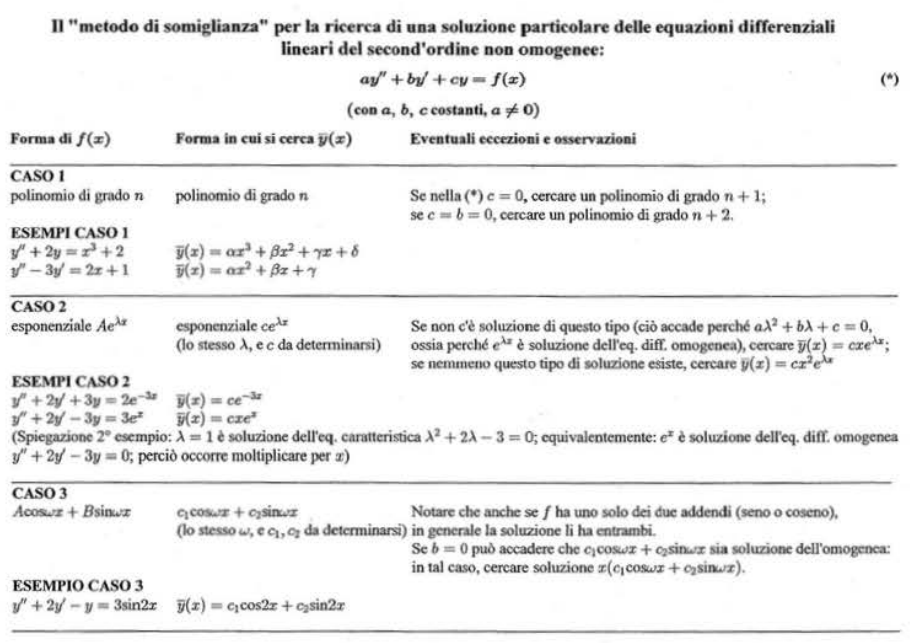
\includegraphics[height=250px]{../img/eqdiff2.PNG}
\end{center}
\begin{center}
    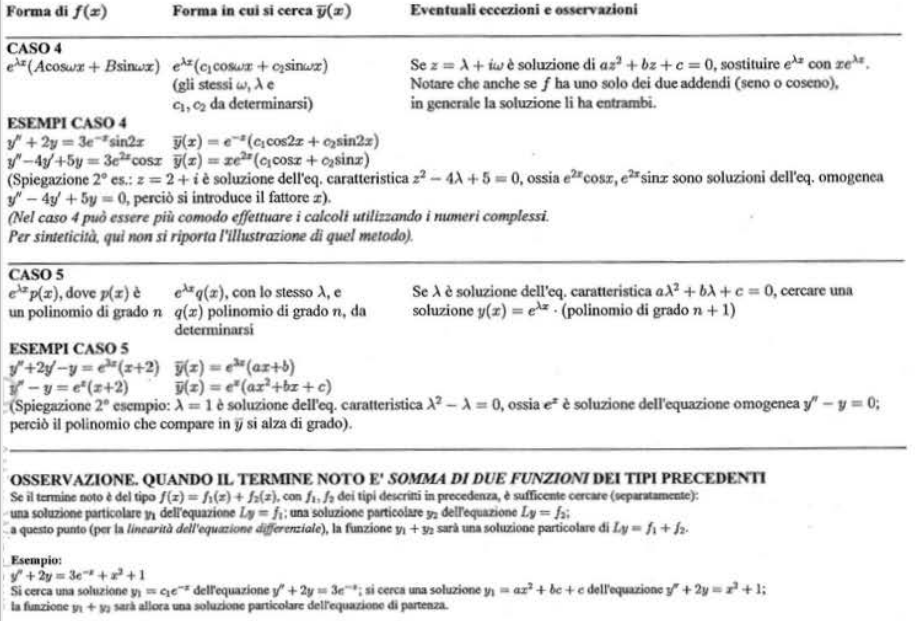
\includegraphics[height=250px]{../img/eqdiff2(1).PNG}
\end{center}
\end{tcolorbox}
\rule{\textwidth}{2pt}
\subsection{Sistemi lineari omogenei}
\[
    y' = A(t) y
\]
viene detto sistema omogeneo.\newline
\[
    \begin{cases}
        y' = A(t) y\\
        y(t_0) = y_0
    \end{cases}
\]
è il problema di cauchy associato.\newline
\newline
Se $y_0 = 0$, allora l'unica soluzione è $y(t) = 0$.\newline
\newline
Se $\phi_1$ e $\phi_2$ risolvono il sistema omogeneo, anche $\alpha \phi_1 + \beta \phi_2$ per ogni $\alpha, \beta \in \mathbb{R}$ lo risolverà.\newline
\newline
Se $A$ è una matrice costante il sistema si dice a coefficienti costanti.\newline
\newline
Sia un matrice $M$, vogliamo calcolare $e^{M}$. \newline
Se $M$ è diagonale si ottiene facilmente:
\[
    M = \left( \begin{matrix}
        \lambda_1  & 0 &\dots & 0\\
        0 & \lambda_2 &\dots &0\\
        0 & 0 &\dots &0\\
        0 & 0 &\dots &\lambda_n
    \end{matrix} \right) \Rightarrow e^M = \left( \begin{matrix}
        e^{\lambda_1}  & 0 &\dots & 0\\
        0 & e^{\lambda_2} &\dots &0\\
        0 & 0 &\dots &0\\
        0 & 0 &\dots & e^{\lambda_n}
    \end{matrix} \right)
\]
Se $M$ non è diagonale, ma è diagonalizzabile, e cioè esiste una matrice non singolare $S$ tale che $\Lambda = S^{-1}MS$ sia diagonale, allora
\[
    M = S\Lambda S^{-1} \Rightarrow  M^k = S\Lambda^kS^{-1} \Rightarrow e^M = S e^{\Lambda}S^{-1}
\]
con $e^{\Lambda}$ che si calcola come abbiamo visto per le matrici diagonali.\newline
\newline
Una matrice quadrata è diagonalizzabile se e solo se tutti i suoi autovalori sono regolari. \newline
\newline
Precisiamo che vengono considerati anche autovalori complessi che, per una matrice a coefficienti reali, possono esserci se e solo se c'è anche il loro coniugato. In tal caso, gli esponenziali dipendenti da tempo vanno interpretati con la formula di Eulero e generano funzioni trigonometriche.\newline
\newline
Abbiamo dunque visto come si trova l'esponenziale di una matrice diagonalizzabile costante. Volendo trovare l'esponenziale della matrice $At$, facciamo un paio di osservazioni elementari:
\begin{itemize}
    \item se A è diagonalizzabile, lo è anche $At$ e si può usare la stessa mtrice di passaggio $S$ per diagonalizzarla
    \item gli autovali di $At$ sono uguali agli autovalori di $A$ moltiplicati per $t$
\end{itemize}
Da queste osservazioni possiamo dedurre che
\[
    e^A  S e^{\Lambda}S^{-1} \Rightarrow  e^{At} = S e^{\Lambda t} S^{-1}
\]
\textbf{teor.} Le colonne della matrice $e^{At}$ formano un sistema fondamentale di soluzioni di $y' = Ay$ e cioè, per ogni $C \in \mathbb{R}^n$ il vettore $e^{At} C$è una soluzione di di $y'=Ay$\newline
\newline
La fuznione $\phi(t) = C e^{\lambda t} $ è soluzione di $y'=At$ se e solo se $\lambda$ è un autovalore di $A$ (possibilmente complesso) e $C$ è un autovettore associato a $\lambda$.\newline
\rule{\textwidth}{0,4pt}
\subsection{Diagonalizzazione di una matrice}
Una matrice $A$ è diagonalizzabile se
\begin{itemize}
    \item Il numero degli autovalori di $A$ contati con la loro molteplicità è uguale all'ordine della matrice
    \item la molteplicità geometrica di ciascun autovalore coincide  con la realtiva molteplicità algebrica
\end{itemize}

Sia $A$ una matrice, i suoi autovalori si ottengono risolvendo
\[
    det(A-\lambda I ) = \left| \begin{matrix}
        a_{11} -\lambda & a_{12}\\
        a_{21} & a_{22} - \lambda
    \end{matrix} \right| = 0
\]
risolvendo questa equazione per $\lambda$ otteniamo i vari autovalori.\newline
La molteplicità algebrica consiste nel quante volte $\lambda$ appare come soluzione dell'equazione precedente.\newline
Perchè $A$ sia diagonalizzabile, la somma della molteplicità algebrica di ogni autovalore deve essere uguale all'ordine della matrice.\newline
Perchè $A$ sia diagonalizzabile bisogna anche verificare che la molteplicità algebrica di ogni autovalore coincide con la realtiva molteplicità geometrica, che si calcola così:
\[
    m_g(\lambda) = n - rk(A- \lambda I)
\]
dove $n$ è l'ordine di $A$.\newline
\newline
\newline
Se $A$ è diagonalizzabile, allora esiste una matrice $P$  che la diagonalizza e una matrice $D$ a cui $A$ è simile, per cui valga:
\[
    D = P A P^{-1}
\]
\begin{itemize}
    \item la matrice $D$ è una matrice diagonale i cui elementi della diagonale principale sono gli autovalori della matrice $A$. Gli autovalori con molteplicità algebrica maggiore di 1 vanno ripetuti più volte.
    \item la matrice $P$ è la matrice che ha come colonne gli autovettori associati a ogni autovalore, ossia ha come colonne i vettori che fromano le basi degli autospazi relativi a ciascun autovalore.
\end{itemize}
Affinchè tutto funzioni ci deve essere corrispondenza fra le matrici $D$ e $P$: la $j$-esima colonna della matrice $P$ contiene l'autovettore associato all'autovalore presente nella $j$-esima colonna della matrice $D$.\newline
\newline
Il calcolo degli autovettori relativi a un autovalore $\lambda$ si esegue risolvendo il sistema:
\[
    (A- \lambda I ) v = 0
\]
con $v = \binom{x}{y}$, e cioè risolvendo il sistema:
\[
    \left(\begin{matrix}
        a_{11} -\lambda & a_{12}\\
        a_{21} & a_{22} - \lambda
    \end{matrix} \right) \binom{x}{y} = 0
\]
\newline
Invece per calcolare l'inversa della matrice $P$ si seguono i seguenti passaggi:
\begin{itemize}
    \item Calcola la trasposta $A^T$ della matrice $A$ (basta scambiare tra loro le righe con le colonne)
    \item sostituire ogni elemento della matrice trasposta col il proprio complemento algebrico (complemento algebrico: preso l'elemento $a_{h,k}$ della matrice, il suo complemento algebrico si calcola come $(-1)^{(h+k)}\cdot C_{h,k}$, dove con $X_{h,k}$ si intende il determinante della matrice ottenuta da quella di partenza eliminando la riga $h$ e la colonna $k$)
    \item Adesso dividi la matrice dei complementi algebrici per det(A) (cioe' dividi ogni termine per det(A)) e ottieni l'inversa della matrice quadrata di partenza
\end{itemize} % equazioni differenziali:
    %- da confrontare con capitolo 7 del libro del prof
    %- aggiugnere capitolo 8 del libro del prof
\end{document}